\documentclass[12pt]{article}
%DIF LATEXDIFF DIFFERENCE FILE


\usepackage[top=1in,left=1in, right = 1in, footskip=1in]{geometry}

\usepackage{graphicx}
\usepackage{xspace}
%\usepackage{adjustbox}

\newcommand{\comment}{\showcomment}
%% \newcommand{\comment}{\nocomment}

\newcommand{\showcomment}[3]{\textcolor{#1}{\textbf{[#2: }\textsl{#3}\textbf{]}}}
\newcommand{\nocomment}[3]{}

\newcommand{\jd}[1]{\comment{cyan}{JD}{#1}}
\newcommand{\swp}[1]{\comment{magenta}{SWP}{#1}}
\newcommand{\bmb}[1]{\comment{blue}{BMB}{#1}}
\newcommand{\djde}[1]{\comment{red}{DJDE}{#1}}

\newcommand{\eref}[1]{Eq.~(\ref{eq:#1})}
\newcommand{\fref}[1]{Fig.~\ref{fig:#1}}
\newcommand{\Fref}[1]{Fig.~\ref{fig:#1}}
\newcommand{\sref}[1]{Sec.~\ref{#1}}
\newcommand{\frange}[2]{Fig.~\ref{fig:#1}--\ref{fig:#2}}
\newcommand{\tref}[1]{Table~\ref{tab:#1}}
\newcommand{\tlab}[1]{\label{tab:#1}}
\newcommand{\seminar}{SE\mbox{$^m$}I\mbox{$^n$}R}

\usepackage{amsthm}
\usepackage{amsmath}
\usepackage{amssymb}
\usepackage{amsfonts}
\usepackage[utf8]{inputenc} % make sure fancy dashes etc. don't get dropped

\usepackage{lineno}
\linenumbers

\usepackage[pdfencoding=auto, psdextra]{hyperref}

\usepackage{natbib}
\bibliographystyle{chicago}
\date{\today}

\usepackage{xspace}
\newcommand*{\ie}{i.e.\@\xspace}

\usepackage{color}

\newcommand{\Rx}[1]{\ensuremath{{\mathcal R}_{#1}}\xspace} 
\newcommand{\Ro}{\Rx{0}}
\newcommand{\Rc}{\Rx{\mathrm{c}}}
%DIF 51a51
\newcommand{\Rs}{\Rx{\mathrm{s}}} %DIF > 
%DIF -------
\newcommand{\RR}{\ensuremath{{\mathcal R}}\xspace}
\newcommand{\Rhat}{\ensuremath{{\hat\RR}}}
\newcommand{\Rintrinsic}{\ensuremath{{\mathcal R}_{\textrm{\tiny intrinsic}}}\xspace}
\newcommand{\tsub}[2]{#1_{{\textrm{\tiny #2}}}}
\newcommand{\dd}[1]{\ensuremath{\, \mathrm{d}#1}}
\newcommand{\dtau}{\dd{\tau}}
\newcommand{\dx}{\dd{x}}
\newcommand{\dsigma}{\dd{\sigma}}

\newcommand{\psymp}{\ensuremath{p}} %% primary symptom time
\newcommand{\ssymp}{\ensuremath{s}} %% secondary symptom time
\newcommand{\pinf}{\ensuremath{\alpha_1}} %% primary infection time
\newcommand{\sinf}{\ensuremath{\alpha_2}} %% secondary infection time

\newcommand{\psize}{{\mathcal P}} %% primary cohort size
\newcommand{\ssize}{{\mathcal S}} %% secondary cohort size

\newcommand{\gtime}{\tau_{\rm g}} %% generation interval
\newcommand{\gdist}{g} %% generation-interval distribution
\newcommand{\idist}{\ell} %% incubation period distribution

\newcommand{\total}{{\mathcal T}} %% total number of serial intervals

\usepackage{lettrine}

\newcommand{\dropcapfont}{\fontfamily{lmss}\bfseries\fontsize{26pt}{28pt}\selectfont}
\newcommand{\dropcap}[1]{\lettrine[lines=2,lraise=0.05,findent=0.1em, nindent=0em]{{\dropcapfont{#1}}}{}}
%DIF PREAMBLE EXTENSION ADDED BY LATEXDIFF
%DIF UNDERLINE PREAMBLE %DIF PREAMBLE
\RequirePackage[normalem]{ulem} %DIF PREAMBLE
\RequirePackage{color}\definecolor{RED}{rgb}{1,0,0}\definecolor{BLUE}{rgb}{0,0,1} %DIF PREAMBLE
\providecommand{\DIFaddtex}[1]{{\protect\color{blue}\uwave{#1}}} %DIF PREAMBLE
\providecommand{\DIFdeltex}[1]{{\protect\color{red}\sout{#1}}}                      %DIF PREAMBLE
%DIF SAFE PREAMBLE %DIF PREAMBLE
\providecommand{\DIFaddbegin}{} %DIF PREAMBLE
\providecommand{\DIFaddend}{} %DIF PREAMBLE
\providecommand{\DIFdelbegin}{} %DIF PREAMBLE
\providecommand{\DIFdelend}{} %DIF PREAMBLE
%DIF FLOATSAFE PREAMBLE %DIF PREAMBLE
\providecommand{\DIFaddFL}[1]{\DIFadd{#1}} %DIF PREAMBLE
\providecommand{\DIFdelFL}[1]{\DIFdel{#1}} %DIF PREAMBLE
\providecommand{\DIFaddbeginFL}{} %DIF PREAMBLE
\providecommand{\DIFaddendFL}{} %DIF PREAMBLE
\providecommand{\DIFdelbeginFL}{} %DIF PREAMBLE
\providecommand{\DIFdelendFL}{} %DIF PREAMBLE
%DIF HYPERREF PREAMBLE %DIF PREAMBLE
\providecommand{\DIFadd}[1]{\texorpdfstring{\DIFaddtex{#1}}{#1}} %DIF PREAMBLE
\providecommand{\DIFdel}[1]{\texorpdfstring{\DIFdeltex{#1}}{}} %DIF PREAMBLE
\newcommand{\DIFscaledelfig}{0.5}
%DIF HIGHLIGHTGRAPHICS PREAMBLE %DIF PREAMBLE
\RequirePackage{settobox} %DIF PREAMBLE
\RequirePackage{letltxmacro} %DIF PREAMBLE
\newsavebox{\DIFdelgraphicsbox} %DIF PREAMBLE
\newlength{\DIFdelgraphicswidth} %DIF PREAMBLE
\newlength{\DIFdelgraphicsheight} %DIF PREAMBLE
% store original definition of \includegraphics %DIF PREAMBLE
\LetLtxMacro{\DIFOincludegraphics}{\includegraphics} %DIF PREAMBLE
\newcommand{\DIFaddincludegraphics}[2][]{{\color{blue}\fbox{\DIFOincludegraphics[#1]{#2}}}} %DIF PREAMBLE
\newcommand{\DIFdelincludegraphics}[2][]{% %DIF PREAMBLE
\sbox{\DIFdelgraphicsbox}{\DIFOincludegraphics[#1]{#2}}% %DIF PREAMBLE
\settoboxwidth{\DIFdelgraphicswidth}{\DIFdelgraphicsbox} %DIF PREAMBLE
\settoboxtotalheight{\DIFdelgraphicsheight}{\DIFdelgraphicsbox} %DIF PREAMBLE
\scalebox{\DIFscaledelfig}{% %DIF PREAMBLE
\parbox[b]{\DIFdelgraphicswidth}{\usebox{\DIFdelgraphicsbox}\\[-\baselineskip] \rule{\DIFdelgraphicswidth}{0em}}\llap{\resizebox{\DIFdelgraphicswidth}{\DIFdelgraphicsheight}{% %DIF PREAMBLE
\setlength{\unitlength}{\DIFdelgraphicswidth}% %DIF PREAMBLE
\begin{picture}(1,1)% %DIF PREAMBLE
\thicklines\linethickness{2pt} %DIF PREAMBLE
{\color[rgb]{1,0,0}\put(0,0){\framebox(1,1){}}}% %DIF PREAMBLE
{\color[rgb]{1,0,0}\put(0,0){\line( 1,1){1}}}% %DIF PREAMBLE
{\color[rgb]{1,0,0}\put(0,1){\line(1,-1){1}}}% %DIF PREAMBLE
\end{picture}% %DIF PREAMBLE
}\hspace*{3pt}}} %DIF PREAMBLE
} %DIF PREAMBLE
\LetLtxMacro{\DIFOaddbegin}{\DIFaddbegin} %DIF PREAMBLE
\LetLtxMacro{\DIFOaddend}{\DIFaddend} %DIF PREAMBLE
\LetLtxMacro{\DIFOdelbegin}{\DIFdelbegin} %DIF PREAMBLE
\LetLtxMacro{\DIFOdelend}{\DIFdelend} %DIF PREAMBLE
\DeclareRobustCommand{\DIFaddbegin}{\DIFOaddbegin \let\includegraphics\DIFaddincludegraphics} %DIF PREAMBLE
\DeclareRobustCommand{\DIFaddend}{\DIFOaddend \let\includegraphics\DIFOincludegraphics} %DIF PREAMBLE
\DeclareRobustCommand{\DIFdelbegin}{\DIFOdelbegin \let\includegraphics\DIFdelincludegraphics} %DIF PREAMBLE
\DeclareRobustCommand{\DIFdelend}{\DIFOaddend \let\includegraphics\DIFOincludegraphics} %DIF PREAMBLE
\LetLtxMacro{\DIFOaddbeginFL}{\DIFaddbeginFL} %DIF PREAMBLE
\LetLtxMacro{\DIFOaddendFL}{\DIFaddendFL} %DIF PREAMBLE
\LetLtxMacro{\DIFOdelbeginFL}{\DIFdelbeginFL} %DIF PREAMBLE
\LetLtxMacro{\DIFOdelendFL}{\DIFdelendFL} %DIF PREAMBLE
\DeclareRobustCommand{\DIFaddbeginFL}{\DIFOaddbeginFL \let\includegraphics\DIFaddincludegraphics} %DIF PREAMBLE
\DeclareRobustCommand{\DIFaddendFL}{\DIFOaddendFL \let\includegraphics\DIFOincludegraphics} %DIF PREAMBLE
\DeclareRobustCommand{\DIFdelbeginFL}{\DIFOdelbeginFL \let\includegraphics\DIFdelincludegraphics} %DIF PREAMBLE
\DeclareRobustCommand{\DIFdelendFL}{\DIFOaddendFL \let\includegraphics\DIFOincludegraphics} %DIF PREAMBLE
%DIF END PREAMBLE EXTENSION ADDED BY LATEXDIFF

\begin{document}

\DIFdelbegin %DIFDELCMD < \begin{flushleft}{
%DIFDELCMD < 	\Large
%DIFDELCMD < 	\textbf\newline{
%DIFDELCMD < 		Cohort-based approach to understanding the roles of generation and serial intervals in shaping epidemiological dynamics
%DIFDELCMD < 	}
%DIFDELCMD < }
%DIFDELCMD < %%%
\DIFdelend \DIFaddbegin \begin{flushleft}{
	\Large
	\textbf\newline{
		Forward-looking serial intervals correctly link epidemic growth to reproduction numbers
	}
}
\DIFaddend \newline
\\
Sang Woo Park\textsuperscript{1,*}
Kaiyuan Sun\textsuperscript{2}
David Champredon\textsuperscript{3}
Michael Li\textsuperscript{4}
Benjamin M.\ Bolker\textsuperscript{4,5,6}
David J.\,D.\ Earn\textsuperscript{5,6}
Joshua S.\ Weitz\textsuperscript{7, 8}
Bryan T.\ Grenfell\textsuperscript{1,2,9}
Jonathan Dushoff\textsuperscript{4,5,6}
\\
\bigskip
\textbf{1} Department of Ecology and Evolutionary Biology, Princeton University, Princeton, NJ, USA
\\
\textbf{2} Fogarty International Center, National Institutes of Health, Bethesda, MD, USA
\\
\textbf{3} Department of Pathology and Laboratory Medicine, University of Western Ontario, London, Ontario, Canada
\\
\textbf{4} Department of Biology, McMaster University, Hamilton, ON, Canada
\\
\textbf{5} Department of Mathematics and Statistics, McMaster University, Hamilton, ON, Canada
\\
\textbf{6} M.\,G.\,DeGroote Institute for Infectious Disease Research, McMaster University, Hamilton, ON, Canada
\\
\textbf{7} School of Biological Sciences, Georgia Institute of Technology, Atlanta, GA, USA
\\
\textbf{8} School of Physics, Georgia Institute of Technology, Atlanta, GA, USA
\\
\textbf{9} Woodrow Wilson School of Public and International Affairs, Princeton University, Princeton, NJ, USA
\\
\bigskip

*Corresponding author: swp2@princeton.edu
\bigskip

Disclaimer: The findings and conclusions in this report are those of the authors and do not necessarily represent the official position of the U.S. National Institutes of Health or Department of Health and Human Services.
\end{flushleft}

\pagebreak

\section*{Abstract}

\DIFdelbegin %DIFDELCMD < \dropcap{G}%%%
\DIFdel{eneration intervals and serial intervals are critical quantities for characterizing outbreak dynamics.
Generation intervalscharacterize }\DIFdelend \DIFaddbegin \DIFadd{The reproduction number }\RR \DIFadd{and the growth rate $r$ are critical epidemiological quantities.
They are linked by generation intervals, }\DIFaddend the time between infection and \DIFdelbegin \DIFdel{transmission}\DIFdelend \DIFaddbegin \DIFadd{onward transmission.
Because generation intervals are difficult to observe, epidemiologists often substitute serial intervals}\DIFaddend , \DIFdelbegin \DIFdel{while serial intervalscharacterize }\DIFdelend the time between \DIFdelbegin \DIFdel{the onset of symptoms in a chain of transmission .
They are often used interchangeably, leading to misunderstanding of }\DIFdelend \DIFaddbegin \DIFadd{symptom onset in successive links in a transmission chain.
Recent studies suggest that such substitution biases estimates of }\RR \DIFadd{based on $r$.
Here we explore }\DIFaddend how these intervals \DIFdelbegin \DIFdel{link the epidemic growth rate $r$ and the reproduction number }\DIFdelend \DIFaddbegin \DIFadd{vary over the course of an epidemic, and the implications for }\DIFaddend \RR \DIFdelbegin \DIFdel{.
Generation intervals provide a mechanistic link between $r$ and }\DIFdelend \DIFaddbegin \DIFadd{estimation.
}\emph{\DIFadd{Forward-looking}} \DIFadd{serial intervals, measuring time forward from symptom onset of an infector, correctly describe the renewal process of symptomatic cases and therefore reliably link }\DIFaddend \RR \DIFdelbegin \DIFdel{but are harder to measure via contact tracing.
While serial intervalsare easier to measure from contact tracing, recent studies suggest that the two intervals give different estimates of }%DIFDELCMD < \RR %%%
\DIFdel{from }\DIFdelend \DIFaddbegin \DIFadd{with }\DIFaddend $r$.
\DIFdelbegin \DIFdel{We present a general framework for characterizing epidemiological delays based on cohorts (i.e., a group of individuals that share the same event time , such as symptom onset) and show that }\DIFdelend \DIFaddbegin \DIFadd{In contrast, }\emph{\DIFadd{backward-looking}} \DIFadd{intervals, which measure time backward, and }\DIFaddend \emph{\DIFdelbegin \DIFdel{forward-looking}\DIFdelend \DIFaddbegin \DIFadd{intrinsic}\DIFaddend } \DIFdelbegin \DIFdel{serial }\DIFdelend intervals, which \DIFdelbegin \DIFdel{correctly link }\DIFdelend \DIFaddbegin \DIFadd{neglect population-level dynamics, give incorrect }\DIFaddend \RR \DIFdelbegin \DIFdel{with $r$, are not the same as ``intrinsic'' serial intervals , but instead change with $r$.
We provide }\DIFdelend \DIFaddbegin \DIFadd{estimates.
Forward-looking intervals are affected both by epidemic dynamics and by censoring, changing in complex ways over the course of an epidemic.
We present }\DIFaddend a heuristic method for addressing \DIFdelbegin \DIFdel{potential biases that can arise from not accounting for }\DIFdelend \DIFaddbegin \DIFadd{biases that arise from neglecting }\DIFaddend changes in serial intervals\DIFdelbegin \DIFdel{across cohorts and }\DIFdelend \DIFaddbegin \DIFadd{. 
We }\DIFaddend apply the method to \DIFdelbegin \DIFdel{estimating }\DIFdelend \DIFaddbegin \DIFadd{early (21 January -- 8 February 2020) serial-interval-based estimates of  }\DIFaddend \RR for the COVID-19 outbreak in China \DIFdelbegin \DIFdel{using serial-interval data --- our analysis shows that using incorrectly }\DIFdelend \DIFaddbegin \DIFadd{outside Hubei province; using improperly }\DIFaddend defined serial intervals \DIFdelbegin \DIFdel{can severely bias estimates }\DIFdelend \DIFaddbegin \DIFadd{in this context biases estimates of initial }\RR \DIFadd{by up to a factor of 2.6}\DIFaddend .
This study demonstrates the importance of early \DIFdelbegin \DIFdel{epidemiological investigation through contact tracing }\DIFdelend \DIFaddbegin \DIFadd{contact-tracing efforts }\DIFaddend and provides a \DIFdelbegin \DIFdel{rationale }\DIFdelend \DIFaddbegin \DIFadd{framework }\DIFaddend for reassessing generation intervals, serial intervals, and \RR\ estimates \DIFdelbegin \DIFdel{, }\DIFdelend for COVID-19.

\section*{Significance Statement}

The generation- and serial-interval distributions are key, but different, quantities in outbreak analyses.
Recent theoretical studies suggest that \DIFaddbegin \DIFadd{the }\DIFaddend two distributions give different estimates of the reproduction number \RR \DIFdelbegin \DIFdel{from the }\DIFdelend \DIFaddbegin \DIFadd{as inferred from the observed }\DIFaddend exponential growth rate $r$\DIFdelbegin \DIFdel{;
however, both intervals, by definition, describe disease transmission at the individual level}\DIFdelend .
Here, we show that \DIFaddbegin \DIFadd{estimating }\RR \DIFadd{based on $r$ and }\DIFaddend the serial-interval distribution, \DIFaddbegin \DIFadd{when }\DIFaddend defined from the correct reference time and cohort, gives the same estimate \DIFdelbegin \DIFdel{of }%DIFDELCMD < \RR %%%
\DIFdel{as }\DIFdelend \DIFaddbegin \DIFadd{as using $r$ and }\DIFaddend the generation-interval distribution.
We \DIFdelbegin \DIFdel{then }\DIFdelend apply our framework to serial-interval data from the COVID-19 outbreak in China\DIFdelbegin \DIFdel{.
While our study supports the use of serial-interval }\DIFdelend \DIFaddbegin \DIFadd{, outside Hubei province (January  21--February 8, 2020), revealing systematic biases in prior inference methods.
Our study provides the theoretical basis for practical changes to the principled use of serial interval }\DIFaddend distributions in estimating \RR \DIFdelbegin \DIFdel{, it also reveals necessary changes to the current understanding and applications of serial-interval distribution}\DIFdelend \DIFaddbegin \DIFadd{during epidemics}\DIFaddend .

\pagebreak

\section{Introduction}

The reproduction number \RR is one of the most important characteristics of an emerging epidemic, \DIFdelbegin \DIFdel{including }\DIFdelend \DIFaddbegin \DIFadd{such as }\DIFaddend the current pandemic of coronavirus disease 2019 (COVID-19) \citep{majumder2020early}.
The reproduction number is defined as the average number of secondary cases caused by a primary case\DIFdelbegin \DIFdel{;
the }\DIFdelend \DIFaddbegin \DIFadd{.
The }\DIFaddend value in a fully susceptible population --- the ``basic'' reproduction number \Ro --- allows us to predict the extent to which an infection will spread in the population, and the amount of intervention necessary to eliminate it \DIFdelbegin \DIFdel{\mbox{%DIFAUXCMD
\citep{anderson1991infectious}}\hspace{0pt}%DIFAUXCMD
.
Near the beginning of an outbreak, }\DIFdelend \DIFaddbegin \DIFadd{in simple cases \mbox{%DIFAUXCMD
\citep{anderson1991infectious}}\hspace{0pt}%DIFAUXCMD
.
Since the reproduction number represents an average \mbox{%DIFAUXCMD
\citep{diekmann1990definition, anderson1991infectious}}\hspace{0pt}%DIFAUXCMD
, it fails to capture heterogeneity among individuals or across space.
The reproduction number also fails to provide any information about the time scale of disease transmission.
}

\DIFadd{Estimating the reproduction number }\DIFaddend \RR is often \DIFdelbegin \DIFdel{estimated from the observed }\DIFdelend \DIFaddbegin \DIFadd{challenging.
Direct estimates based on observed infections will typically be biased down when some infections cannot be observed.
A common method of estimating }\RR \DIFadd{near the beginning of an epidemic is based on the population-level }\DIFaddend exponential growth rate \DIFdelbegin \DIFdel{using generation- and serial-interval distributions (e.g., \mbox{%DIFAUXCMD
\cite{wallinga2007generation, fraser2009pandemic, hampson2009transmission, chunara2012social, chowell2014west, du2020serial, jung2020real}}\hspace{0pt}%DIFAUXCMD
) but the differences among two distributions are often neglected.
}%DIFDELCMD < 

%DIFDELCMD < %%%
\DIFdel{The }\DIFdelend \DIFaddbegin \DIFadd{$r$, which can often be estimated robustly from case reports \mbox{%DIFAUXCMD
\citep{mills2004transmissibility, ma2014estimating}}\hspace{0pt}%DIFAUXCMD
.
The growth rate $r$ and the reproduction number }\RR \DIFadd{are linked by the generation-interval distribution \mbox{%DIFAUXCMD
\cite{wallinga2007generation}}\hspace{0pt}%DIFAUXCMD
, where the }\DIFaddend generation interval is defined as the time between when an individual (infector) is infected and when that individual infects another person (infectee) \DIFdelbegin \DIFdel{;
the generation-interval distribution determines the relationship between the exponential growth rate $r$ and the reproduction number }%DIFDELCMD < \RR %%%
\DIFdel{\mbox{%DIFAUXCMD
\citep{anderson1991infectious, ferguson2005strategies, wallinga2007generation}}\hspace{0pt}%DIFAUXCMD
.
Similarly, the serial }\DIFdelend \DIFaddbegin \DIFadd{\mbox{%DIFAUXCMD
\citep{svensson2007note}}\hspace{0pt}%DIFAUXCMD
.
}

\DIFadd{Since generation intervals measure time between infection events, which can be difficult to observe in practice, generation intervals are often replaced with serial intervals.
The serial }\DIFaddend interval is defined as the time between when an infector and an infectee \DIFdelbegin \DIFdel{become }\emph{\DIFdel{symptomatic}} %DIFAUXCMD
\DIFdelend \DIFaddbegin \DIFadd{develop symptoms }\DIFaddend \citep{svensson2007note}.
While \DIFdelbegin \DIFdel{serial intervals are similar to generation intervals, }\DIFdelend \DIFaddbegin \DIFadd{generation and serial intervals both measure the time scale of disease transmission, they measure fundamentally different quantities. 
In particular, }\DIFaddend previous studies have noted that, in many contexts, serial intervals are expected to have larger variances than generation intervals but have the same mean \DIFdelbegin \DIFdel{\mbox{%DIFAUXCMD
\citep{svensson2007note,klinkenberg2011correlation,te2013estimating,champredon2018equivalence}}\hspace{0pt}%DIFAUXCMD
.
}\DIFdelend \DIFaddbegin \DIFadd{in many contexts \mbox{%DIFAUXCMD
\citep{svensson2007note,klinkenberg2011correlation,te2013estimating,champredon2018equivalence}}\hspace{0pt}%DIFAUXCMD
.
Serial intervals can in some cases even take negative values in the presence of presymptomatic transmission \mbox{%DIFAUXCMD
\citep{he2020temporal}}\hspace{0pt}%DIFAUXCMD
, whereas generation intervals must be positive.
}\DIFaddend 

Although these distributions were clearly and distinctly defined over a decade ago \citep{svensson2007note}, 
the need for a better conceptual and theoretical framework for understanding their differences is becoming clearer as the COVID-19 pandemic unfolds.
Researchers continue to \DIFdelbegin \DIFdel{rely }\DIFdelend \DIFaddbegin \DIFadd{base inferences about COVID-19 }\DIFaddend on both generation and serial intervals \DIFdelbegin \DIFdel{to make inferences about COVID-19, either without making a clear distinction \mbox{%DIFAUXCMD
\citep{tempvar,du2020serial,he2020temporal,wu2020nowcasting,zhao2020serial}}\hspace{0pt}%DIFAUXCMD
, or explicitly conflating the two intervals
\mbox{%DIFAUXCMD
\citep{anderson2020will,hellewell2020feasibility}}\hspace{0pt}%DIFAUXCMD
.}\DIFdelend \DIFaddbegin \DIFadd{without clearly distinguishing between them (e.g., \mbox{%DIFAUXCMD
\cite{tempvar,du2020serial,he2020temporal,wu2020nowcasting,zhao2020serial}}\hspace{0pt}%DIFAUXCMD
), and, in some cases, explicitly conflate the definitions of the two intervals (e.g., \mbox{%DIFAUXCMD
\cite{anderson2020will,hellewell2020feasibility}}\hspace{0pt}%DIFAUXCMD
).
This confusion is apparent even in standard software for estimating }\RR\DIFadd{, such as }\texttt{\DIFadd{EpiEstim}}\DIFadd{, in which the serial-interval distribution is used to infer time-dependent }\RR \DIFadd{\mbox{%DIFAUXCMD
\citep{thompson2019improved}}\hspace{0pt}%DIFAUXCMD
.
These studies are examples of many---indeed, it is a common practice to use the serial and generation intervals interchangeably.
}\DIFaddend 

One source of confusion arises from an apparent discrepancy between the \DIFdelbegin \DIFdel{serial-interval and }\DIFdelend generation-interval \DIFdelbegin \DIFdel{viewpoints.
When }\DIFdelend \DIFaddbegin \DIFadd{and serial-interval viewpoints.
While }\DIFaddend the epidemic is growing exponentially, the spread of infection can be characterized as a \emph{renewal process} based on previous incidence of infection, the associated generation-interval distribution, and the average infectiousness of an infected individual.
It is well established that this renewal formulation allows us to link the exponential growth rate of an epidemic $r$ with its reproduction number \RR using the generation-interval distribution \citep{wallinga2007generation}.
\DIFdelbegin \DIFdel{By definition}\DIFdelend \DIFaddbegin \DIFadd{However}\DIFaddend , the serial-interval distribution \DIFdelbegin \DIFdel{describes the renewal process between symptomatic cases based on their symptom onset dates;
since }\DIFdelend \DIFaddbegin \DIFadd{also describes a renewal process --- in this case, the creation of a new }\emph{\DIFadd{symptomatic}} \DIFadd{case based on a symptomatic case in the previous generation.
Since }\DIFaddend both renewal processes, based on \DIFaddbegin \DIFadd{either }\DIFaddend generation- \DIFdelbegin \DIFdel{and }\DIFdelend \DIFaddbegin \DIFadd{or }\DIFaddend serial-interval distributions, describe the same underlying \DIFdelbegin \DIFdel{system of exponential growth}\DIFdelend \DIFaddbegin \DIFadd{exponentially growing system}\DIFaddend , both should provide the same correct link between the reproduction number \RR and the epidemic growth rate $r$.
\DIFaddbegin 

\DIFaddend In contexts where the \DIFdelbegin \DIFdel{distributions are expected to be different}\DIFdelend \DIFaddbegin \DIFadd{serial- and generation-interval distributions differ}\DIFaddend , current theory has no explanation for how \DIFdelbegin \DIFdel{these differing }\DIFdelend \DIFaddbegin \DIFadd{two different }\DIFaddend distributions could provide identical estimates of \RR from $r$. 
\DIFdelbegin \DIFdel{Some studies have further suggested that using serial intervals can underestimate }%DIFDELCMD < \RR %%%
\DIFdel{because the serial-interval distribution is wider than the generation-interval distribution \mbox{%DIFAUXCMD
\citep{britton2019estimation, ganyani2020estimating}}\hspace{0pt}%DIFAUXCMD
.
}\DIFdelend \DIFaddbegin \DIFadd{In fact, recent theory suggest that using the serial-interval can underestimate the reproduction number \mbox{%DIFAUXCMD
\citep{britton2019estimation, ganyani2020estimating}}\hspace{0pt}%DIFAUXCMD
.
However, these studies rely on }\emph{\DIFadd{intrinsic}} \DIFadd{distributions of incubation periods and generation intervals that neglect the population-level dynamics of disease spread.
}\DIFaddend 

Here \DIFdelbegin \DIFdel{, we resolve this apparent discrepancy by showing thatthe relevant interval for the renewal framework is what is called the }\DIFdelend \DIFaddbegin \DIFadd{we show that, by correctly defining and calculating the }\DIFaddend ``forward'' \DIFdelbegin \DIFdel{interval, and that the forward serial }\DIFdelend \DIFaddbegin \DIFadd{serial-interval distribution (i.e., a distribution of serial intervals from a cohort of infectors that developed symptoms at the same time) that connects symptom onset dates, we can resolve this discrepancy.
These forward }\DIFaddend intervals are different from the ``intrinsic'' serial intervals that previous studies have relied on \citep{svensson2007note,klinkenberg2011correlation,te2013estimating,champredon2018equivalence, britton2019estimation}.
\DIFaddbegin \DIFadd{During an ongoing epidemic, all observed epidemiological delays (e.g., incubation period) between primary (e.g., infection) and secondary (e.g., symptom onset) events are subject to backward biases: when the incidence of primary events is increasing (or decreasing), we are more likely to observe shorter (respectively longer) intervals.
In particular, when we consider forward serial-interval distributions, the incubation periods of the infectors are subject to backward biases because we have to look backward in time from their symptom onset to infection.
Therefore, the realized incubation period distributions of the infector and the infectee can differ dynamically, even if the intrinsic analogues of the same distributions are expected to be equivalent.
}

\DIFaddend We develop a \DIFdelbegin \DIFdel{new }\DIFdelend \DIFaddbegin \DIFadd{cohort-based }\DIFaddend framework for characterizing and comparing \DIFaddbegin \DIFadd{realized }\DIFaddend serial intervals, as well as any other epidemiological delays, and show that the initial forward serial-interval distribution correctly estimates \RR from $r$.
Conversely, using inaccurately defined serial intervals or failing to account for changes in the observed serial-interval distributions over the course of an epidemic can considerably bias estimates of \RR.
\DIFdelbegin \DIFdel{We apply our framework to serial intervals of COVID-19 and }\DIFdelend \DIFaddbegin \DIFadd{For example, in our analysis of the COVID-19 serial intervals from China, outside Hubei province, we find that the original }\Ro \DIFadd{estimates based on aggregated serial-interval data underestimated }\Ro \DIFadd{by a factor of 2.0--2.6.
We further }\DIFaddend lay out several principles to consider in using information about serial intervals and other epidemiological time delays to correctly infer the \DIFaddbegin \DIFadd{initial }\DIFaddend reproduction number during the early stages of an outbreak.

\section{Methods}

\subsection{Intrinsic, forward, and backward delay distributions}

\DIFdelbegin \DIFdel{The time delays }\DIFdelend \DIFaddbegin \DIFadd{A time delay }\DIFaddend between two epidemiological events can \DIFdelbegin \DIFdel{be defined either within an }\DIFdelend \DIFaddbegin \DIFadd{involve either one }\DIFaddend infected individual (e.g., incubation period: infection and symptom onset of an individual) or \DIFdelbegin \DIFdel{between infected individuals }\DIFdelend \DIFaddbegin \DIFadd{two --- an infector and an infectee }\DIFaddend (e.g., \DIFdelbegin \DIFdel{serial interval: symptom onsets of an infector and an infectee}\DIFdelend \DIFaddbegin \DIFadd{generation and serial intervals}\DIFaddend ).
We \DIFdelbegin \DIFdel{can further divide these events into }\DIFdelend \DIFaddbegin \DIFadd{define the delay as the time difference between the }\DIFaddend \emph{primary} \DIFdelbegin \DIFdel{and }\DIFdelend \DIFaddbegin \DIFadd{event and the }\DIFaddend \emph{secondary} \DIFdelbegin \DIFdel{events.
When we measure an epidemiological time delay within an infected individual (e.g., the incubation period), the primary event usually }\DIFdelend \DIFaddbegin \DIFadd{event.
In some cases, the primary event always }\DIFaddend occurs before the secondary event \DIFdelbegin \DIFdel{---
most epidemiological events that can be observed within an individual have clear direction }\DIFdelend (e.g., \DIFaddbegin \DIFadd{the time from }\DIFaddend infection to onset of symptoms \DIFdelbegin \DIFdel{) but some may not }\DIFdelend \DIFaddbegin \DIFadd{in a single individual, or the generation interval between two individuals). 
In other cases, the delay can sometimes be negative }\DIFaddend (e.g., \DIFaddbegin \DIFadd{the time from }\DIFaddend onset of infectiousness \DIFdelbegin \DIFdel{and }\DIFdelend \DIFaddbegin \DIFadd{to }\DIFaddend onset of symptoms \DIFdelbegin \DIFdel{).
When we measure an epidemiological time delay between infected individuals (e.g., }\DIFdelend \DIFaddbegin \DIFadd{in a single individual, or }\DIFaddend the serial interval \DIFdelbegin \DIFdel{), 
the primary and secondary events are defined in terms of the direction of transmission:
the primary event refers to the event that occurs in the infector.
Again, some of these delays are always positive (the infector is always infected before the infectee) and some are not (it is possible for the infectee to develop symptoms before the infector \mbox{%DIFAUXCMD
\citep{he2020temporal}}\hspace{0pt}%DIFAUXCMD
).
}\DIFdelend \DIFaddbegin \DIFadd{between two individuals).
}\DIFaddend 

At the individual level, we can define the time distribution between a primary and a secondary event that we expect to observe \DIFdelbegin \DIFdel{(averaged across individual characteristics) for an infected individual }\DIFdelend \DIFaddbegin \DIFadd{for a single infected individual by averaging across individual characteristics }\DIFaddend --- we refer to this distribution as the \DIFdelbegin \DIFdel{intrinsic distribution}\DIFdelend \DIFaddbegin \emph{\DIFadd{intrinsic distribution}}\DIFaddend .
For example, the intrinsic incubation period distribution describes the expected time distribution from infection to symptom onset of an infected individual.
Likewise, the intrinsic generation-interval distribution describes the expected time distribution of infectious contacts made by an infected individual.
However, the intrinsic time distributions are not always equivalent to the corresponding realized time distributions at the population level (i.e., the distribution of time between actual primary and secondary events that occur during an epidemic\DIFaddbegin \DIFadd{; see \fref{diagram}}\DIFaddend ).
For example, an infectious contact results in infection only if the contacted individual is susceptible (and has not already been infected) \DIFdelbegin \DIFdel{;
}\DIFdelend \DIFaddbegin \DIFadd{---
}\DIFaddend this is one mechanism that causes realized generation intervals (time between actual infection events) to differ from from the intrinsic generation intervals (time between infection and infectious contacts) \DIFdelbegin \DIFdel{.
}\DIFdelend \DIFaddbegin \DIFadd{\mbox{%DIFAUXCMD
\citep{park2020inferring}}\hspace{0pt}%DIFAUXCMD
.
In this example, the difference between intrinsic and realized time distributions can be attributed to the fact that the fraction of susceptible individuals is itself dynamic.
}\DIFaddend 

At the population level, we model realized time delays between a primary and a secondary event from a cohort perspective.
A cohort consists of \DIFdelbegin \emph{\DIFdel{all}} %DIFAUXCMD
\DIFdelend \DIFaddbegin \DIFadd{all }\DIFaddend individuals whose (primary or secondary) event occurred at a given time.
%DIF > % \psymp, \ssymp have \ensuremath in def so don't need $$ when used in isolation
For example, when we are measuring incubation periods, a primary cohort consists of all individuals who became infected at time \psymp, while a secondary cohort consists of all individuals whose symptom onset occurred at time \DIFdelbegin \DIFdel{$\ssymp$}\DIFdelend \DIFaddbegin \ssymp\DIFaddend .
Similarly, when we are measuring serial intervals, a primary cohort consists of all infectors who became symptomatic at time \DIFdelbegin \DIFdel{$\psymp$}\DIFdelend \DIFaddbegin \psymp\DIFaddend .
Then, for \DIFaddbegin \DIFadd{a }\DIFaddend primary cohort at time \DIFdelbegin \DIFdel{$\psymp$}\DIFdelend \DIFaddbegin \psymp\DIFaddend , we can define the \DIFdelbegin \DIFdel{expected time distribution }\DIFdelend \DIFaddbegin \DIFadd{distribution of realized delays }\DIFaddend between primary and secondary events. 
We refer to this distribution as the forward delay distribution and denote it as $f_\psymp(\tau)$.

Likewise, we define the backward delay distribution $b_\ssymp(\tau)$ for a secondary cohort at time \DIFdelbegin \DIFdel{$\ssymp$}\DIFdelend \DIFaddbegin \ssymp\DIFaddend :
The backward delay distribution describes the time delays between a primary and secondary \DIFdelbegin \DIFdel{host }\DIFdelend \DIFaddbegin \DIFadd{events }\DIFaddend given that the secondary event occurred at time \DIFdelbegin \DIFdel{$\ssymp$}\DIFdelend \DIFaddbegin \ssymp\DIFaddend .
For example, the backward incubation period distribution at time \DIFdelbegin \DIFdel{$\ssymp$ }\DIFdelend \DIFaddbegin \ssymp\DIFadd{\ }\DIFaddend describes incubation periods for a \emph{cohort} of individuals who became symptomatic at time \DIFdelbegin \DIFdel{$\ssymp$}\DIFdelend \DIFaddbegin \ssymp\DIFaddend .
Likewise, the backward serial-interval distribution at time \DIFdelbegin \DIFdel{$\ssymp$ }\DIFdelend \DIFaddbegin \ssymp\DIFadd{\ }\DIFaddend describes serial intervals for a \emph{cohort} of infectees who became symptomatic at time \DIFdelbegin \DIFdel{$\ssymp$}\DIFdelend \DIFaddbegin \ssymp\DIFaddend .

Both forward and backward perspectives
must yield identical \emph{measurement} (e.g., the length of the incubation
period of a given individual is the same whether measured forward from
the time of infection or backward from the time of symptom onset).
%DIF <  Consequently, if we restrict attention to individuals with a given
%DIF <  incubation period, say $\tau$ days, and we count how many became infected at time $\psymp$
%DIF <  or how many first showed symptoms at time $\ssymp=\psymp+\tau$ then we must obtain
%DIF <  the same number. 
Consequently, no matter how delays are distributed, if
$\mathcal P$ and $\mathcal S$ represent the sizes of primary and
secondary cohorts then we can express the total density of intervals \DIFdelbegin \DIFdel{between time $\psymp$ and $\ssymp$ }\DIFdelend \DIFaddbegin \DIFadd{$\tau$ between calendar time }\psymp\DIFadd{\ and }\ssymp\DIFadd{\ (i.e., $\tau=\ssymp-\psymp$) }\DIFaddend as follows:
\begin{equation}
W(\psymp) \psize(\psymp) f_\psymp(\tau) = \ssize(\ssymp) b_\ssymp(\tau) \,,
\label{eq:match}
\end{equation}
where $W(\psymp)$, the ``weight'' of the primary cohort, represents the average number of forward intervals that an individual in cohort $\psize(\psymp)$ produces over the course of their infection.
When we measure within-individual delays, we expect $W(\psymp) \leq 1$ because only a subset of individuals who experience the primary event (e.g., infection) will eventually experience the secondary event (e.g., symptom onset).
For between-individual delays, we expect $W(\psymp)$ to change throughout an epidemic, because individuals infected earlier in an epidemic will infect more individuals on average than those infected later.

Substituting $\psymp=\ssymp-\tau$, it follows that
\begin{equation}
b_\ssymp(\tau)= \frac{W(\ssymp-\tau) \psize(\ssymp-\tau) f_{\ssymp-\tau} (\tau)}{\ssize(\ssymp)}\,.
\label{eq:backward}
\end{equation}
If we are considering incubation periods, the left hand side of
this equation is the probability density that an individual
who became symptomatic at time \DIFdelbegin \DIFdel{$\ssymp$ }\DIFdelend \DIFaddbegin \ssymp\DIFadd{\ }\DIFaddend had an incubation period of
length $\tau$.
From the right hand side, we see that this probability density depends on the weight parameter \DIFdelbegin \DIFdel{$W(\psymp-\tau)$ }\DIFdelend \DIFaddbegin \DIFadd{$W(\ssymp-\tau)$ }\DIFaddend (in this case, the proportion of symptomatic infection),
the time-varying primary cohort size at the earlier time $\psize(\ssymp-\tau)$ (in this case, the number of individuals infected at time $\ssymp-\tau$),
and the forward delay distribution $f_{\ssymp-\tau}(\tau)$ (in this case, the probability density that an incubation period that starts at time $\ssymp-\tau$ ends at time \DIFdelbegin \DIFdel{$\ssymp$}\DIFdelend \DIFaddbegin \ssymp\DIFaddend ).

Several different mechanisms drive the changes in forward and backward delay distributions over time.
Typically, within-individual forward delay distributions are not directly affected by epidemic dynamics.
Some realized \DIFaddbegin \DIFadd{forward }\DIFaddend distributions, like incubation period distributions, are \DIFdelbegin \DIFdel{expected to be }\DIFdelend equivalent to their intrinsic distributions and remain invariant at the time scale of an outbreak.
Other realized distributions, like the distribution of time from symptom onset to testing, may change over the course of an epidemic due to changes in \DIFdelbegin \DIFdel{public health policies }\DIFdelend \DIFaddbegin \DIFadd{public-health policies or individual behavior}\DIFaddend .
Between-individual forward delay distributions, such as generation- or serial-interval distributions, depend on epidemic dynamics\DIFdelbegin \DIFdel{;
for }\DIFdelend \DIFaddbegin \DIFadd{.
For }\DIFaddend example, forward generation intervals \DIFdelbegin \DIFdel{contract during the outbreak because infected individuals are less likely to infect others later in the epidemic due to factors that drive time-dependent decreases in transmission such as }\DIFdelend \DIFaddbegin \DIFadd{often become shorter as an epidemic progresses due to the dynamical process of }\DIFaddend susceptible depletion, \DIFdelbegin \DIFdel{behavioral change, and interventions \mbox{%DIFAUXCMD
\citep{champredon2015intrinsic}}\hspace{0pt}%DIFAUXCMD
}\DIFdelend \DIFaddbegin \DIFadd{as well as due to other factors like behavioral change or interventions \mbox{%DIFAUXCMD
\citep{kenah2008generation, nishiura2010time, champredon2015intrinsic}}\hspace{0pt}%DIFAUXCMD
: if it is harder to infect later in the course of infection, then proportionally more intervals will be short}\DIFaddend .

\eref{backward} suggests that backward delay distributions change over time even if their corresponding forward delay distribution does not change.
Backward delay distributions depend on changes in the primary cohort size over time due to conditionality of observations:
Conditioning on individuals whose secondary events have occurred at the same time means that we tend to observe shorter (or longer) inter-event delays when cohort size has been increasing (decreasing) through time.
When incidence is growing exponentially, we can calculate the amount of bias exactly.
Assuming that the forward delay distribution ($f_\psymp(\tau) \approx f_0(\tau)$) and the weight parameter ($W(\psymp) \approx W(0)$) remain constant during the exponential growth phase, we can substitute $\psize(t) = \psize(0) \exp(rt)$ in \eref{backward} to obtain:
\begin{align}
b_0(\tau) &= \left[ W(0) \psize(0)/\ssize(0)\right] \exp(-r\tau) f_0(\tau)
\label{eq:backexp}
\end{align}
where $r$ is the exponential growth rate\DIFdelbegin \DIFdel{(and $\left[W(0) \psize(0)/\ssize(0)\right]^{-1} = \int_{-\infty}^{\infty} \exp(-r\tau') f_0(\tau') \dtau'$ since }\DIFdelend \DIFaddbegin \DIFadd{.
Since }\DIFaddend $b_0$ is a probability distribution\DIFdelbegin \DIFdel{).
Thus, for faster epidemics (higher $r$), }\DIFdelend \DIFaddbegin \DIFadd{, $\left[W(0) \psize(0)/\ssize(0)\right]^{-1} = \int_{-\infty}^{\infty} \exp(-r\tau') f_0(\tau') \dtau'$ corresponds to the normalization constant.
Therefore, }\DIFaddend the backward delay distribution \DIFdelbegin \DIFdel{will have a shorter mean}\DIFdelend \DIFaddbegin \DIFadd{during the exponential growth phase depends only on the exponential growth rate $r$ and the initial forward delay distribution $f_0$}\DIFaddend .
\DIFaddbegin 

\DIFadd{The mean backward interval will be always shorter than the mean forward interval as long as $r > 0$.
Even for different epidemics of the same disease, we expect to observe shorter backward intervals within a fast-growing epidemic (high $r$), all else being equal.
}\DIFaddend In general, the backward delay distribution will differ from the forward delay distribution (unless the disease is at equilibrium), even if we are measuring time delays that are intrinsic to the life history of a disease (e.g., the incubation period).
These ideas apply to all epidemiological delay distributions and generalize the work by \cite{champredon2015intrinsic} who compared forward and backward generation-interval distributions to describe realized generation intervals from the perspective of an infector and an infectee, respectively, as well as the work by \cite{britton2019estimation} who showed that \eref{backexp} holds for the backward generation-interval \DIFdelbegin \DIFdel{distributions}\DIFdelend \DIFaddbegin \DIFadd{distribution}\DIFaddend .

\subsection{Realized serial-interval distributions}

The serial interval is defined as the time between when an infector becomes symptomatic and when \DIFdelbegin \DIFdel{an }\DIFdelend \DIFaddbegin \DIFadd{their }\DIFaddend infectee becomes symptomatic \citep{svensson2007note}.
Previous studies have often expressed serial intervals $\tau_{\rm s}$ in the form (\fref{diagram}A):
\begin{equation}
\tau_{\rm s} = (\gtime + \tau_{\rm i2}) - \tau_{\rm i1}
\label{eq:intser}
\end{equation}
where $\tau_{\rm i1}$ and $\tau_{\rm i2}$ represent incubation periods of an infector and
an infectee, respectively, and $\gtime$ represents the generation
interval between the infector and the infectee.
These studies \DIFdelbegin \DIFdel{assume that $\tau_{\rm i1}$ and $\tau_{\rm i2}$ are drawn from the same distributions and }\DIFdelend concluded that the serial and generation intervals have the same mean \DIFdelbegin \DIFdel{\mbox{%DIFAUXCMD
\citep{svensson2007note,klinkenberg2011correlation,champredon2018equivalence, britton2019estimation}}\hspace{0pt}%DIFAUXCMD
;
however, this conclusion is based on the implicit assumption that }\DIFdelend \DIFaddbegin \DIFadd{when $\tau_{\rm i1}$ and $\tau_{\rm i2}$ are drawn from the same distributions \mbox{%DIFAUXCMD
\citep{svensson2007note,klinkenberg2011correlation,champredon2018equivalence, britton2019estimation}}\hspace{0pt}%DIFAUXCMD
.
However, }\DIFaddend distributions of realized incubation periods, $\tau_{\rm i1}$ and $\tau_{\rm i2}$ \DIFdelbegin \DIFdel{, as well as generation interval, $\gtime$, }\DIFdelend \DIFaddbegin \DIFadd{will be identical only if we assume that they }\DIFaddend are intrinsic to individuals (and not dependent on epidemic dynamics at the population-level) ---
something that is generally true of forward but not backward incubation-period distributions.
We refer to the definition \eref{intser} as the intrinsic serial interval (\fref{diagram}A).

\begin{figure}[!th]
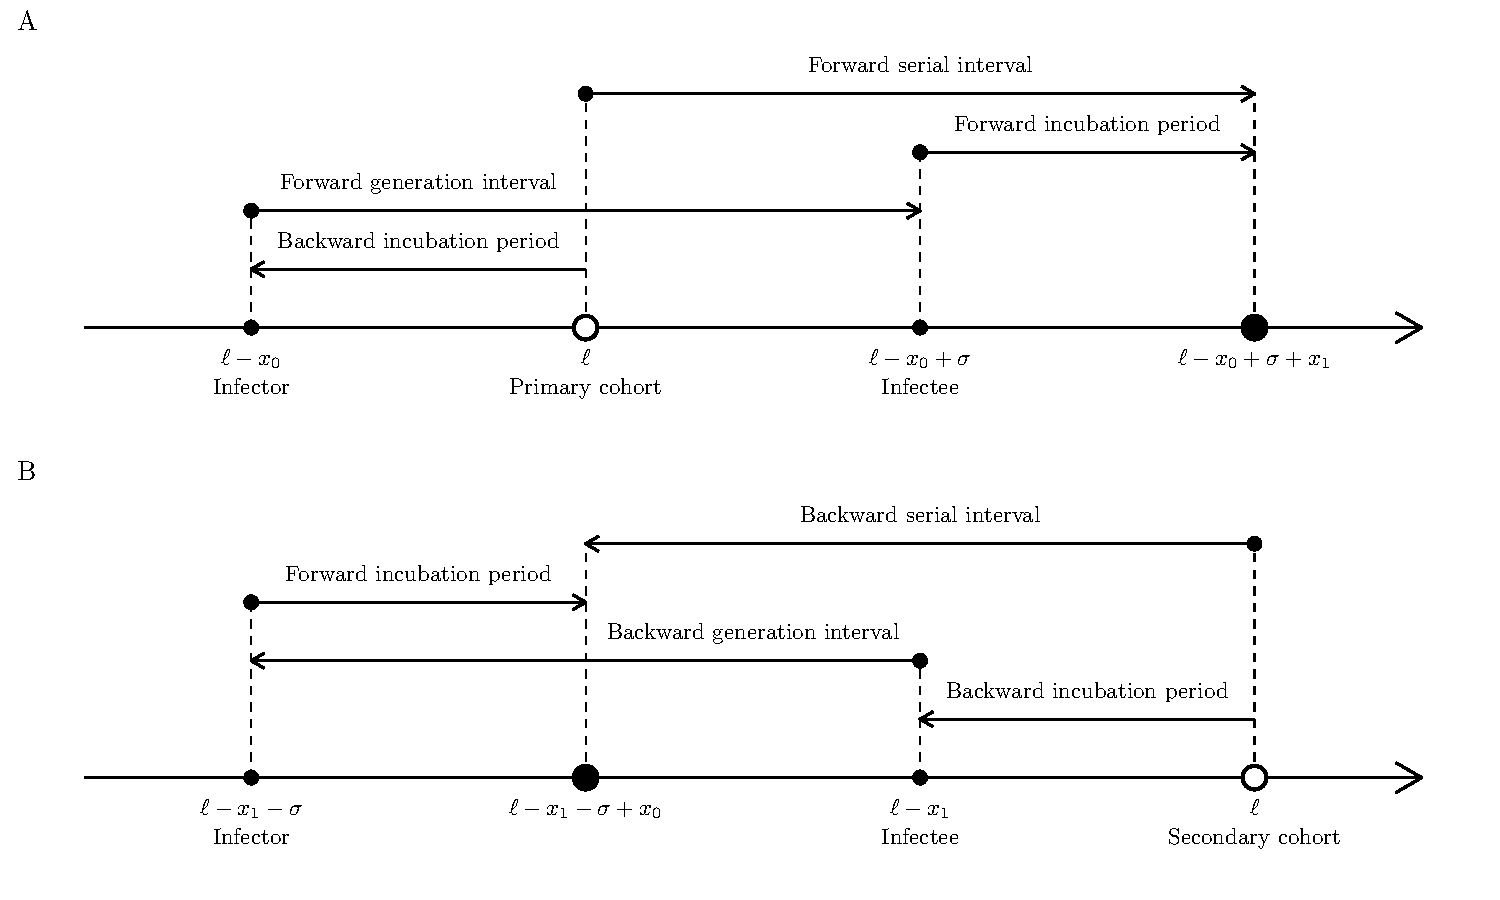
\includegraphics[width=\textwidth]{serial_guide.pdf}
\caption{
\textbf{Illustration of intrinsic,
    forward and backward serial intervals.}  (A) The intrinsic serial
  interval for a cohort of individuals infected at time $\psymp$.  In
  this case, $\tau_{\rm i1}$ is drawn from the intrinsic incubation period
  distribution; $\gtime$ is drawn from the intrinsic generation-interval
  distribution; and $\tau_{\rm i2}$ is drawn from the intrinsic incubation period
  distribution.  (B) The forward serial interval for a cohort of
  infectors who became symptomatic at time $\psymp$.  In this case,
  $\tau_{\rm i1}$ is drawn from the backward incubation period distribution; $\gtime$
  is drawn from the forward generation-interval distribution; and $\tau_{\rm i2}$
  is drawn from the forward incubation period distribution.  (C) The
  backward serial interval for a cohort of infectees who became
  symptomatic at time \DIFdelbeginFL \DIFdelFL{$\ssymp$}\DIFdelendFL \DIFaddbeginFL \ssymp\DIFaddendFL .  In this case, $\tau_{\rm i1}$ is drawn from the
  forward incubation period distribution; $\gtime$ is drawn from the
  backward generation-interval distribution; and $\tau_{\rm i2}$ is drawn from the
  backward incubation period distribution.
  \DIFaddbeginFL \DIFaddFL{Intrinsic intervals (black) reflect average of individual characteristics and are not dependent on population-level dynamics.
  Forward intervals (green) can change due to epidemiological dynamics (e.g., contraction of generation intervals through susceptible depletion).
  Backward intervals (blue) can change due to changes in cohort sizes even when forward intervals remain time-invariant.
}\DIFaddendFL }
\label{fig:diagram}
\end{figure}

To correctly link the realized serial-interval distribution to the renewal process
between cases based on symptom onset dates, we must use the forward
serial interval (i.e., use the perspective of a cohort of infectors
that share the same symptom onset time).  Given that an infector
became symptomatic at time $\psymp$, to calculate the forward serial
interval we first go \DIFdelbegin \DIFdel{backward }\DIFdelend \DIFaddbegin \emph{\DIFadd{backward}} \DIFaddend in time to when the infector was
infected, and then forward in time to when the infectee was infected,
and then forward \DIFaddbegin \DIFadd{again }\DIFaddend to when the infectee became symptomatic.
In \fref{diagram}B, we see that $\tau_{\rm i1}$ is drawn from
the backward incubation period distribution of the cohort
of infectors who became symptomatic at time $\psymp$; $\gtime$ is drawn from
the forward generation-interval distribution of the cohort of
infectors who became infected at time $\psymp - \tau_{\rm i1}$; and $\tau_{\rm i2}$
is drawn from the forward incubation period distribution of the cohort of
infectees who became infected at time $\psymp - \tau_{\rm i1} + \gtime$.
Likewise, we can define the backward serial-interval distribution for
a cohort of infectees who became symptomatic at time \DIFdelbegin \DIFdel{$\ssymp$
}\DIFdelend \DIFaddbegin \ssymp
\DIFaddend (\fref{diagram}C).  
This conceptual framework demonstrates that the distributions of $\tau_{\rm i1}$, $\gtime$, and $\tau_{\rm i2}$ (and therefore the distributions of realized serial intervals) depend on the reference cohort, which is defined by \DIFdelbegin \DIFdel{an event type (primary or secondary),
}\DIFdelend temporal direction (forward or backward) \DIFdelbegin \DIFdel{, }\DIFdelend and a particular reference time.

To calculate realized serial-interval distributions, we begin by modeling $\total(\psymp,\ssymp)$: the total density of serial intervals that start (when infectors develop symptoms) at time $\psymp$ and end (when infectees develop symptoms) at time \DIFdelbegin \DIFdel{$\ssymp$.
The }\DIFdelend \DIFaddbegin \ssymp\DIFadd{.
For simplicity, we assume that all infected individuals eventually develop symptoms.
Then, the }\DIFaddend density of serial intervals between time $\psymp$ and \DIFdelbegin \DIFdel{$\ssymp$}\DIFdelend \DIFaddbegin \ssymp\DIFaddend ,
given that the infectors became infected at time $\pinf\le\psymp$ and
the infectees became infected at time $\sinf\le\ssymp$, depends on the
amount of infection that occurs between time $\pinf$ and $\sinf$ as well as
the density of forward incubation periods between $\pinf$ and
$\psymp$ (realized incubation periods of infectors) and between
$\sinf$ and \DIFdelbegin \DIFdel{$\ssymp$ }\DIFdelend \DIFaddbegin \ssymp \DIFaddend (realized incubation periods of infectees):
\begin{equation}
\DIFaddbegin \DIFadd{\total (}\psymp\DIFadd{,}\ssymp \DIFadd{| \alpha_1, \alpha_2)=}\DIFaddend \underbrace{\Rc (\pinf)}_{\substack{\text{case} \\ \text{reproduction} \\ \text{number}}} 
\times 
\underbrace{i(\pinf)}\DIFdelbegin \DIFdel{_{\text{incidence}} 
}\DIFdelend \DIFaddbegin \DIFadd{_{\substack{\text{incidence} \\ \text{of} \\ \text{infection}}} 
}\DIFaddend \times 
\underbrace{h_{\pinf}(\psymp-\pinf, \sinf - \pinf)}\DIFdelbegin \DIFdel{_{\substack{\text{joint density of} \\ \text{the forward incubation} \\ \text{period } p-\pinf \text{ and the forward} \\ \text{generation interval } \sinf-\pinf\\ \text{(of infectors)}}}
}\DIFdelend \DIFaddbegin \DIFadd{_{\substack{\text{joint density of} \\ \text{forward incubation} \\ \text{periods } p-\pinf \text{ and forward} \\ \text{generation intervals } \sinf-\pinf\\ \text{(of infectors)}}}
}\DIFaddend \times
\underbrace{\idist_{\sinf}(\ssymp - \sinf)}\DIFdelbegin \DIFdel{_{\substack{\text{marginal density of} \\ \text{the forward incubation} \\ \text{period } \ssymp-\sinf \\ \text{(of infectees)}}}}\DIFdelend \DIFaddbegin \DIFadd{_{\substack{\text{marginal density of} \\ \text{forward incubation} \\ \text{periods } \ssymp-\sinf \\ \text{(of infectees)}}}}\DIFaddend ,
\end{equation}
where the case reproduction number $\Rc (\pinf)$ is defined as the average number of secondary cases \DIFdelbegin \DIFdel{caused by }\DIFdelend \DIFaddbegin \DIFadd{that }\DIFaddend a primary case infected at time $\pinf$ \DIFaddbegin \DIFadd{will generate }\DIFaddend over the course of their infection \citep{fraser2007estimating}.
We describe the forward incubation periods and the forward generation intervals using a joint probability distribution because onset of symptoms and transmission potential jointly depend on the life history of a disease;
for example, if an infected individual can only transmit the disease after symptom onset, the forward generation interval will necessarily be longer than the forward incubation period.

The total \DIFdelbegin \DIFdel{amount }\DIFdelend \DIFaddbegin \DIFadd{density }\DIFaddend of serial intervals \DIFaddbegin \DIFadd{between time $\psymp$ and $\ssymp$ }\DIFaddend can now be obtained by integrating over all possible infection times for the infector and the infectee:
\begin{equation}
\total (\psymp,\ssymp) = \int_{-\infty}^{\psymp} \int_{\pinf}^{\ssymp} \DIFdelbegin %DIFDELCMD < \Rc %%%
\DIFdelend \DIFaddbegin \DIFadd{\total }\DIFaddend (\DIFdelbegin %DIFDELCMD < \pinf%%%
\DIFdel{) i(}%DIFDELCMD < \pinf%%%
\DIFdel{) h_{\pinf}(}\DIFdelend \psymp\DIFdelbegin \DIFdel{-}%DIFDELCMD < \pinf%%%
\DIFdelend ,\DIFdelbegin %DIFDELCMD < \sinf %%%
\DIFdel{- }%DIFDELCMD < \pinf%%%
\DIFdel{) \idist_{\sinf}(}\DIFdelend \ssymp \DIFdelbegin \DIFdel{- }%DIFDELCMD < \sinf%%%
\DIFdelend \DIFaddbegin \DIFadd{| \alpha_1, \alpha_2}\DIFaddend ) \, \mathrm{d}\sinf\,\mathrm{d}\pinf.
\end{equation}
Then, the forward serial-interval distribution $f_\psymp(\tau)$ is given by the density of intervals of length $\tau$ starting at \DIFaddbegin \DIFadd{time }\DIFaddend \psymp, relative to the total number of serial intervals starting at \DIFaddbegin \DIFadd{time }\DIFaddend \psymp: 
\begin{equation}
f_\psymp(\tau) = 
\frac{\total(\psymp, \psymp+\tau)}{\int_{-\infty}^\infty \total(\psymp, \psymp+\tau') \dtau'}.
\label{eq:fserial}
\end{equation}
Likewise, the backward serial-interval distribution $b_\ssymp(\tau)$ is given by the density of intervals of length $\tau$ ending at \ssymp, relative to the total number of serial intervals ending at \ssymp: 
\begin{equation}
b_\ssymp(\tau) = 
\frac{\total(\ssymp-\tau, \ssymp)}{\int_{-\infty}^\infty \total(\ssymp-\tau', \ssymp) \dtau'}.
\label{eq:bserial}
\end{equation}
\DIFaddbegin 

\DIFadd{The denominator of the forward serial-interval distribution (\eref{fserial}) then corresponds to the total number of infections generated by primary cases who themselves developed symptoms at time }\psymp\DIFadd{.
Dividing this quantity by the number of individuals who developed symptoms at time }\psymp\DIFadd{, $j(\psymp) = \int_{-\infty}^\infty \total(\psymp-\tau', \psymp) \dtau'$, we obtain the serial reproduction number:
}\begin{equation}
\DIFadd{\Rs(\psymp) = \frac{\int_{-\infty}^\infty \total(\psymp, \psymp+\tau') \dtau'}{j(\psymp)},
}\end{equation}
\DIFadd{which we define as the average number of infections generated by an individual who developed symptoms at time }\psymp\DIFadd{.
Combining the forward serial-interval distribution with the serial reproduction number completes the renewal process between symptomatic cases:
}\begin{equation}
\DIFadd{j(t) = \int_{-\infty}^\infty \Rs(t-\tau) j(t-\tau) f_{t-\tau}(\tau) \dtau.
\label{eq:jrenew}
}\end{equation}
\DIFaddend This framework allows us to understand changes in the realized serial intervals for any \DIFdelbegin \DIFdel{deterministic epidemic model .
}\DIFdelend \DIFaddbegin \DIFadd{epidemic model and properly link serial-interval distributions with the renewal process.
In addition,  assuming that the reproduction number as well as the forward serial-interval distribution remain constant during the exponential growth phase, we can substitute $j(t) \approx j(0) \exp(rt)$, $\Rs(t) \approx \Rs(0)$, and $f_{t-\tau}(\tau) \approx f_0(\tau)$ to obtain:
}\begin{equation}
\DIFadd{\frac{1}{\Rs(0)} = \int_{-\infty}^\infty \exp(-r\tau) f_{0}(\tau) \mathrm{d} \tau.
\label{eq:Rforward0}
}\end{equation}
\DIFadd{Therefore, the initial forward serial-interval distribution, $f_0(\tau)$, provides the correct link between the exponential growth rate $r$ and the initial serial reproduction number $\Rs(0)$.
We re-visit this idea later in Section 2.4 and show that the initial forward serial-interval distribution provides the same $r$--}\RR \DIFadd{link as the intrinsic generation-interval distribution.
}\DIFaddend 

\subsection{Epidemic model}

We illustrate changes in \DIFdelbegin \DIFdel{the }\DIFdelend forward and backward serial intervals over the course of an epidemic by applying \DIFdelbegin \DIFdel{it }\DIFdelend \DIFaddbegin \DIFadd{our framework }\DIFaddend to a specific example of an epidemic model.
We model disease spread with a renewal-equation model \citep{heesterbeek1996concept, diekmann2000mathematical, roberts2004modelling, aldis2005integral, roberts2007model, champredon2018equivalence}.
Ignoring births and deaths, changes in the proportion of susceptible individuals $S(t)$ and incidence of infection $i(t)$ can be \DIFdelbegin \DIFdel{written as:
}\DIFdelend \DIFaddbegin \DIFadd{described as:
}\DIFaddend \begin{align}
\frac{\mathrm{d}S}{\mathrm{d}t} &= - i(t)\nonumber\\
i(t) &= \DIFdelbegin %DIFDELCMD < \Ro %%%
\DIFdel{S}\DIFdelend \DIFaddbegin \RR\DIFaddend (t) \int_0^\infty i(t-\tau) \gdist(\tau) \dtau,
\label{eq:renewal}
\end{align}
where \DIFdelbegin %DIFDELCMD < \Ro %%%
\DIFdel{is the basic reproduction number , }\DIFdelend \DIFaddbegin \DIFadd{$\RR(t)$ is the instantaneous reproduction number (i.e., the average number of secondary cases that a primary case infected at time $t$ will generate if conditions at time $t$ remain unchanged \mbox{%DIFAUXCMD
\citep{fraser2007estimating}}\hspace{0pt}%DIFAUXCMD
), }\DIFaddend and $\gdist(\tau)$ is the intrinsic generation-interval distribution (i.e., the forward generation-interval distribution of a primary case in a population where \DIFdelbegin \DIFdel{the number of susceptibles remains constant)}\DIFdelend \DIFaddbegin \DIFadd{changes in $\RR(t)$ is negligible \mbox{%DIFAUXCMD
\citep{champredon2015intrinsic}}\hspace{0pt}%DIFAUXCMD
).
This model assumes that $g(\tau)$ remains constant through time -- in other words, that epidemic dynamics are driven by changes in transmission rate. 
This assumption may not be well suited to individual-based intervention such as case isolation \mbox{%DIFAUXCMD
\citep{fraser2007estimating}}\hspace{0pt}%DIFAUXCMD
;
nonetheless, this form has been widely used in the literature and has been successfully applied in modeling the current COVID-19 pandemic \mbox{%DIFAUXCMD
\citep{gostic2020practical}}\hspace{0pt}%DIFAUXCMD
.
}

\DIFadd{Here, changes in reproduction number can be modeled as a product of the basic reproduction number $\Ro$, proportion susceptible $S(t)$, and a time-dependent factor $M(t)$ (for example, accounting for nonpharmaceutical interventions and behavioral changes): $\RR(t) = \Ro S(t) M(t)$;
\mbox{%DIFAUXCMD
\cite{flaxman2020estimating} }\hspace{0pt}%DIFAUXCMD
used a similar framework to evaluate the impact of nonpharmaceutical interventions on the spread of COVID-19 in 11 countries}\DIFaddend .
Then, the forward generation-interval for a cohort of individuals that were infected at time $\psymp$ follows \citep{champredon2015intrinsic}:
\begin{equation}
\gdist_\psymp (\tau) = \DIFdelbegin \DIFdel{\frac{ \gdist(\tau) S(\psymp + \tau)}{\int_0^\infty \gdist(\tau') S(\psymp + \tau') \dtau'}}\DIFdelend \DIFaddbegin \DIFadd{\frac{ \gdist(\tau) S(\psymp + \tau) M(\psymp + \tau) }{\int_0^\infty \gdist(\tau') S(\psymp + \tau') M(\psymp + \tau') \dtau'}}\DIFaddend ,
\end{equation}
which allows us to separate the joint probability distribution $h_\psymp$ of the forward incubation period and the forward generation-interval distribution as a product of the proportion of susceptible individuals $S$ and the joint probability distribution $h$ of the forward incubation period and the intrinsic generation intervals:
\begin{equation}
h_\psymp (x, \tau) = \DIFdelbegin \DIFdel{\frac{h(x, \tau) S(\psymp + \tau)}{\int_0^\infty \int_0^\infty h(x', \tau') S(\psymp + \tau') \dtau' \dx'}}\DIFdelend \DIFaddbegin \DIFadd{\frac{h(x, \tau) S(\psymp + \tau) M(\psymp + \tau)}{\int_0^\infty \int_0^\infty h(x', \tau') S(\psymp + \tau') M(\psymp + \tau') \dtau' \dx'}}\DIFaddend .
\end{equation}
We further assume that the forward incubation period distribution does
not vary across cohorts over the course of an epidemic, as it
represents the life history of a disease; we denote it as $\idist$.
Then, we have:
\begin{align}
\idist(x) &= \int_0^\infty h(x, \tau) \dtau\nonumber\DIFaddbegin \DIFadd{,}\DIFaddend \\
\gdist(\tau) &= \int_0^\infty h(x, \tau) \dx\DIFaddbegin \DIFadd{.
}\DIFaddend \label{eq:marginal}
\end{align}
Finally, the case reproduction for this model is defined as follows:
\begin{equation}
\Rc(t) = \Ro \int_0^\infty \gdist(\tau) S(t+\tau) \DIFaddbegin \DIFadd{M(}\psymp \DIFadd{+ \tau) }\DIFaddend \dtau.
\end{equation}
The forward and backward serial-interval distributions are then calculated by substituting these quantities into \eref{fserial} and \eref{bserial}.
We use this framework to illustrate how the realized epidemiological time distributions vary over the course of an epidemic and depend on the perspective (i.e., forward vs. backward).

\DIFaddbegin \DIFadd{For simplicity, we let $M = 1$ and assume that epidemic dynamics depend only on susceptible depletion in our simulations.
Since we are interested in the initial epidemic growth phase (i.e., linking $r$ to }\RR\DIFadd{), we expect $\RR(t)$ to remain roughly constant during this period.
In addition, qualitative effects of $M$ that reduces $\RR(t)$ monotonically over time will be similar to the impact of susceptible depletion under this modeling framework. 
Therefore, general conclusions we draw from our analysis is expected to be robust---however, detailed shape of the epidemic curve and changes in generation- and serial-intervals can still depend on the shape of $M$.
}

\DIFaddend \subsection{Linking $r$ and \RR}

During the initial phase of an epidemic, the proportion susceptible remains approximately constant ($S(t) \approx S(0)$) and incidence of infection grows exponentially: $i(t) \approx i_0\exp(rt)$.
During this period, the intrinsic generation-interval distribution provides the correct link between the exponential growth rate $r$ and the initial reproduction number $\RR=\Ro S(0)$ based on the Euler-Lotka equation \citep{wallinga2007generation}.
Here, we focus on the estimates of the basic reproduction number \Ro (the value of \RR in a fully susceptible population, $S(t) \approx 1$):
\begin{equation}
\frac{1}{\Ro} = \int_0^\infty \exp(-r\tau) g(\tau) \dtau.
\label{eq:Rgen}
\end{equation}
Analogous to the intrinsic generation-interval distribution, 
forward serial-interval distributions describe the renewal process \DIFdelbegin \DIFdel{of infection based on symptom onset dates}\DIFdelend \DIFaddbegin \DIFadd{between symptomatic cases}\DIFaddend .
Therefore, we expect the forward serial-interval distribution during the exponential growth phase --- which we refer to as the \emph{initial} forward serial-interval distribution $f_0$ --- to estimate the same value of \Ro for a given $r$ as the intrinsic generation-interval distribution (note, however, that the forward serial interval is not necessarily positive):
\begin{equation}
\frac{1}{\Ro} = \int_{-\infty}^\infty \exp(-r\tau) f_{0}(\tau) \mathrm{d} \tau\DIFdelbegin \DIFdel{,
}\DIFdelend \DIFaddbegin \DIFadd{.
}\DIFaddend \label{eq:Rforward}
\end{equation}
\DIFdelbegin \DIFdel{where }\DIFdelend \DIFaddbegin \DIFadd{Here, }\DIFaddend the initial forward serial-interval distribution is given by:
\begin{equation}
f_{0}(\tau) = \frac{1}{\phi} \int_{-\infty}^{0} \int_{\pinf}^{\tau} \exp(r \pinf) h(-\pinf, \sinf - \pinf) \idist(\tau - \sinf) \, \mathrm{d}\sinf\,\mathrm{d}\pinf,
\label{eq:initialSI}
\end{equation}
where the normalization constant $\phi$ is determined by the requirement that $\int_{-\infty}^\infty f_{0}(\tau)\,\dtau=1$.
\DIFdelbegin \DIFdel{In Supplementary Materials, we }\DIFdelend \DIFaddbegin \DIFadd{We }\DIFaddend provide a mathematical proof of this relationship \DIFdelbegin \DIFdel{.
}\DIFdelend \DIFaddbegin \DIFadd{in Supplementary Materials.
Since we do not make any assumptions about the shape of the joint distribution $h$ between incubation periods and the generation intervals, \eref{Rforward} holds in general whether or not there is a presymptomatic transmission period.
}

\DIFaddend We further compare this with the estimate of \Ro based on the intrinsic serial-interval distribution $q(\tau)$:
\begin{equation}
\frac{1}{\Rintrinsic} = \int_{-\infty}^\infty \exp(-r\tau) q(\tau) \mathrm{d} \tau.
\label{eq:Rintrinsic}
\end{equation}
\DIFdelbegin \DIFdel{Here, the }\DIFdelend \DIFaddbegin \DIFadd{The }\DIFaddend intrinsic serial-interval distribution $q(\tau)$ does not depend on epidemic dynamics\DIFaddbegin \DIFadd{, and is given by}\DIFaddend :
\begin{equation}
q(\tau) = \frac{1}{\phi_q} \int_{-\infty}^{0} \int_{\pinf}^{\tau} h(-\pinf, \sinf - \pinf) \idist(\tau - \sinf) \, \mathrm{d}\sinf\,\mathrm{d}\pinf,
\label{eq:intrinsicSI}
\end{equation}
where the normalization constant $\phi_q$ is determined by the
requirement that $\int_{-\infty}^\infty q(\tau)\,\dtau=1$.
Rather than numerically integrating over closed forms of $g$, $f_0$, and $q$ to estimate $\Ro$, we use simulation-based approaches for simplicity (Supplementary Materials).

The initial forward serial-interval distribution depends on the exponential growth rate $r$.
For a fast-growing epidemic (high $r$), we expect the backward incubation periods to be short (\eref{backexp}), \DIFdelbegin \DIFdel{and therefore, the }\DIFdelend \DIFaddbegin \DIFadd{meaning that presymptomatic transmission is less likely to occur. 
Therefore, the initial }\DIFaddend forward serial-interval distribution will generally have a larger mean than the intrinsic generation- and serial-interval distributions.
\DIFdelbegin \DIFdel{The }\DIFdelend \DIFaddbegin \DIFadd{However, the exact shape of the initial forward serial-interval distribution depends on the shape of the joint distribution.
For example, the }\DIFaddend Susceptible-Exposed-Infected-Recovered model, under the additional assumption that the incubation and exposed periods are equivalent (i.e. that onset of symptoms and infectiousness occur simultaneously), provides a special case\DIFdelbegin \DIFdel{where }\DIFdelend \DIFaddbegin \DIFadd{.
In this case, }\DIFaddend the forward serial- and generation-intervals follow the same distributions during the exponential growth phase because (i) infected individuals can only transmit after symptom onset and (ii) the time between symptom onset and infection is independent of the incubation period of an infector (see Supplementary Materials).
\DIFaddbegin \DIFadd{Everywhere else in this paper, however, we do not assume that the incubation and exposed periods are equivalent.
Instead, we allow for presymptomatic transmission in the model in order to reflect the transmission dynamics of COVID-19.
}\DIFaddend 

\subsection{Model parameterization}

We \DIFdelbegin \DIFdel{parameterize our model based on parameter estimates for COVID-19 (Table 1).
We }\DIFdelend \DIFaddbegin \DIFadd{have shown that the dynamics of the serial-interval distribution depend on the joint distribution between incubation periods and generation intervals.
Here, we }\DIFaddend use a bivariate lognormal distribution to model the joint probability distribution \DIFdelbegin \DIFdel{of the }\DIFdelend \DIFaddbegin \DIFadd{$h$ of }\DIFaddend intrinsic incubation periods and \DIFdelbegin \DIFdel{the }\DIFdelend intrinsic generation intervals \DIFaddbegin \DIFadd{(in the renewal equation model, \eref{renewal}) }\DIFaddend while allowing for the possibility that they might be correlated.
\DIFaddbegin \DIFadd{Given that the viral load of SARS-CoV-2 peaks around the time of symptom onset \mbox{%DIFAUXCMD
\citep{he2020temporal}}\hspace{0pt}%DIFAUXCMD
, we generally expect the generation intervals to be positively correlated with the incubation period:
that is, individuals who develop symptoms later are more likely to transmit later.
Marginal distributions of incubation periods and generation intervals are parameterized based on parameter estimates for COVID-19 (Table 1).
}\DIFaddend For simplicity, we consider \DIFdelbegin \DIFdel{three }\DIFdelend \DIFaddbegin \DIFadd{four }\DIFaddend values for the correlation coefficients (on the log scale) of the bivariate lognormal distribution: \DIFdelbegin \DIFdel{$\rho = -0.5, 0, 0.5$.
}\DIFdelend \DIFaddbegin \DIFadd{$\rho = 0, 0.25, 0.5, 0.75$.
This parameterization allows for generation intervals to be shorter than the incubation period, allowing for presymptomatic transmission.
}\DIFaddend 

\begin{table}[!ht]
\begin{center}
\begin{tabular}{|l|l|r|}
\hline
Parameter & Values & Source\\
\hline
Mean intrinsic incubation period & 5.5 days & \cite{lauer2020incubation} \\
SD intrinsic incubation period & 2.4 days & \cite{lauer2020incubation} \\
Mean intrinsic generation interval & \DIFdelbeginFL \DIFdelFL{5 }\DIFdelendFL \DIFaddbeginFL \DIFaddFL{5.0 }\DIFaddendFL days & \cite{ferretti2020quantifying} \\
SD intrinsic generation interval & \DIFdelbeginFL \DIFdelFL{2 }\DIFdelendFL \DIFaddbeginFL \DIFaddFL{1.9 }\DIFaddendFL days & \cite{ferretti2020quantifying} \\
\hline
\end{tabular}
\end{center}
\caption{
  \textbf{Parameter values used for simulations.}
The intrinsic \DIFdelbeginFL \DIFdelFL{generation-interval }\DIFdelendFL \DIFaddbeginFL \DIFaddFL{incubation period }\DIFaddendFL distribution is parameterized using a log-normal distribution with log mean \DIFdelbeginFL \DIFdelFL{$\mu_G=1.54$ }\DIFdelendFL \DIFaddbeginFL \DIFaddFL{$\mu_I=1.62$ }\DIFaddendFL and log standard deviation \DIFdelbeginFL \DIFdelFL{$\sigma_G=0.37$}\DIFdelendFL \DIFaddbeginFL \DIFaddFL{$\sigma_I=0.42$}\DIFaddendFL .
The intrinsic \DIFdelbeginFL \DIFdelFL{incubation period }\DIFdelendFL \DIFaddbeginFL \DIFaddFL{generation-interval }\DIFaddendFL distribution is parameterized using a log-normal distribution with log mean \DIFdelbeginFL \DIFdelFL{$\mu_I=1.62$ }\DIFdelendFL \DIFaddbeginFL \DIFaddFL{$\mu_G=1.54$ }\DIFaddendFL and log standard deviation \DIFdelbeginFL \DIFdelFL{$\sigma_I=0.42$}\DIFdelendFL \DIFaddbeginFL \DIFaddFL{$\sigma_G=0.37$}\DIFaddendFL .
\DIFaddbeginFL \DIFaddFL{Log mean and log standard deviations represent the mean and standard deviations of the underlying normal distributions, which are later exponentiated.
}\DIFaddendFL The joint probability distribution is modeled using a bivariate log-normal distribution with correlations (on the log scale) \DIFdelbeginFL \DIFdelFL{$\rho=-0.5, 0, 0.5$}\DIFdelendFL \DIFaddbeginFL \DIFaddFL{$\rho=\{0, 0.25, 0.5, 0.75\}$}\DIFaddendFL .
The intrinsic  \DIFdelbeginFL \DIFdelFL{generation-interval and }\DIFdelendFL incubation period \DIFaddbeginFL \DIFaddFL{and generation-interval }\DIFaddendFL distributions are chosen to match characteristic of COVID-19 to illustrate realistic magnitudes of time-varying/perspective effects in the current pandemic.
}
\end{table}

\section{Results}

We use parameter estimates for COVID-19 to characterize the degree to which the realized serial-interval distribution can change over the course of \DIFdelbegin \DIFdel{the epidemic and }\DIFdelend \DIFaddbegin \DIFadd{an epidemic and to }\DIFaddend evaluate how different definitions of the serial-interval distribution can affect the Euler-Lotka estimates of \Ro.
We further address how the observed serial intervals, measured through contact tracing, are affected by \DIFdelbegin \DIFdel{the }\DIFdelend right censoring during an ongoing epidemic and provide a heuristic method for addressing biases that can arise from using \DIFdelbegin \DIFdel{serial interval }\DIFdelend \DIFaddbegin \DIFadd{serial-interval }\DIFaddend data to estimate \Ro. 
Finally, we analyze \DIFdelbegin \DIFdel{the serial interval }\DIFdelend \DIFaddbegin \DIFadd{serial-interval }\DIFaddend data from the COVID-19 epidemic in China\DIFaddbegin \DIFadd{, outside Hubei province, based on 468 transmission events reported between January 21--February 8, 2020, }\DIFaddend under our framework.

\subsection{Realized serial-interval distributions \DIFaddbegin \DIFadd{during the exponential growth phase}\DIFaddend }

\fref{rR} shows Euler-Lotka estimates of \Ro\ \DIFaddbegin \DIFadd{based }\DIFaddend on different definitions of the serial interval. 
When the initial forward serial-interval \DIFdelbegin \DIFdel{distributions }\DIFdelend \DIFaddbegin \DIFadd{distribution }\DIFaddend $f_0(\tau)$ is used, estimates (from \eref{Rforward}) exactly match the (correct) generation-interval-based estimates (\eref{Rgen}) for all values of the correlation $\rho$ between the intrinsic incubation period and the intrinsic generation interval (\fref{rR}A).
When the intrinsic distributions are used, however, estimates based on the serial interval (\eref{Rintrinsic}) underestimate \Ro: as $r$ increases, \Rintrinsic saturates and eventually \emph{decreases} due to the increasing inferred importance of negative serial intervals (\fref{rR}B).
While the initial forward serial intervals during the exponential growth phase can also be negative, their effects are appropriately balanced because faster epidemic growth leads to longer serial intervals (and a corresponding lower proportion of negative intervals).

\begin{figure}[!th]
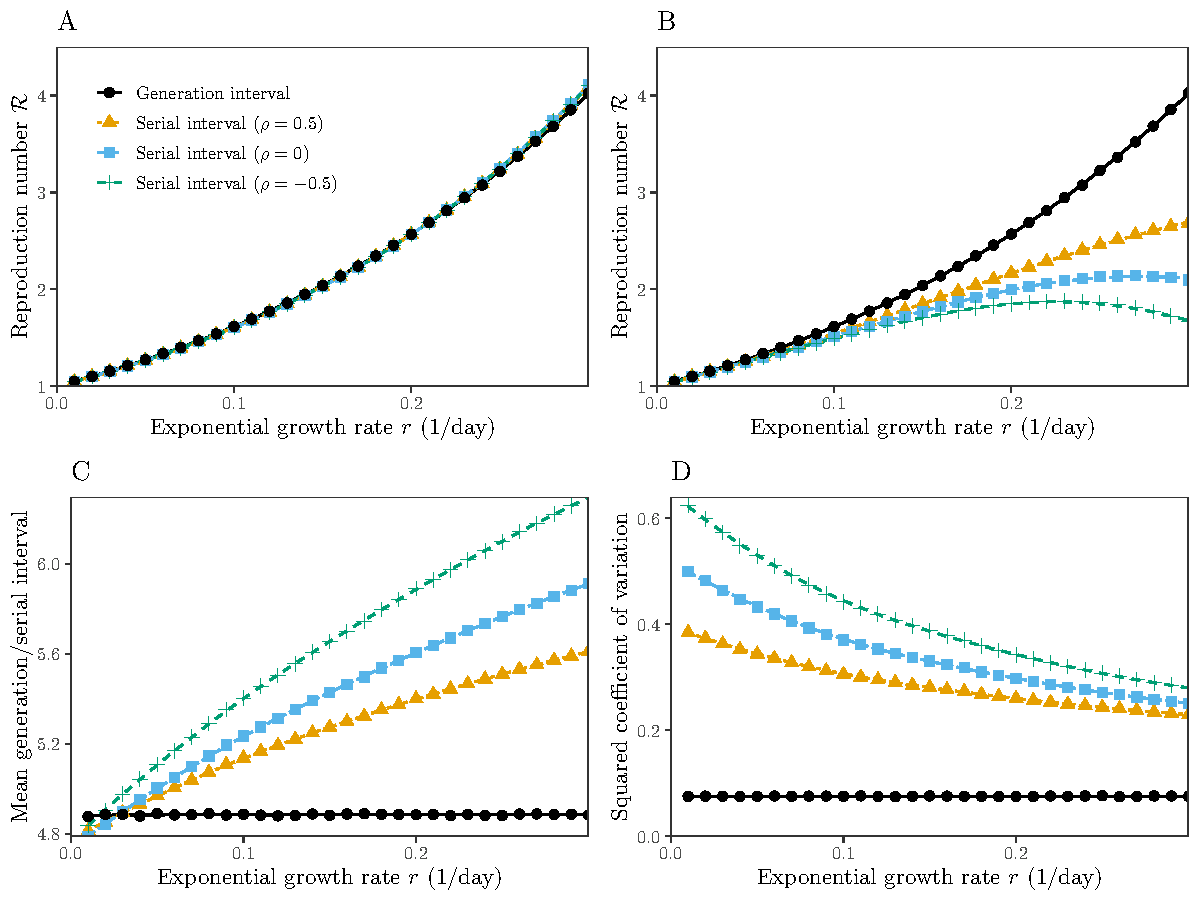
\includegraphics[width=\textwidth]{rR.pdf}
\caption{
\textbf{Estimates of the reproduction number from the exponential growth rate based on serial- and generation-interval distributions.}
(A). The initial forward serial-interval distributions give \DIFdelbeginFL \DIFdelFL{a }\DIFdelendFL \DIFaddbeginFL \DIFaddFL{the }\DIFaddendFL correct
link between the exponential growth rate $r$ and the reproduction
number \Ro,
for any correlation $\rho$ between intrinsic incubation period and
intrinsic generation interval of the underlying bivariate log-normal distribution.
(B) The intrinsic serial-interval distributions give an incorrect link between $r$ and \Ro.
(C) The mean initial forward serial interval during the exponential growth phase increases with $r$.
(D) The squared coefficient of variation of the initial forward serial intervals during the exponential growth phase decreases with $r$.
}
\label{fig:rR}
\end{figure}

Comparing the shapes of the initial forward serial-interval distribution (\eref{initialSI}) and the intrinsic generation-interval distribution allows us to better understand how different forward distributions lead to identical estimates of \Ro.
In general, distributions with higher means and less variability lead to higher \Ro for a given $r$ \citep{wallinga2007generation, weitz2015modeling, park2019practical}.
When incidence is growing exponentially, forward serial intervals have higher means (\fref{rR}C) and squared coefficients of variation (\fref{rR}D) than the intrinsic generation-interval distribution.
The effects of higher means (which increase \Ro) exactly cancel those of higher variability (which decrease \Ro).
On the other hand, \emph{intrinsic} serial intervals (\eref{intrinsicSI}) have the same mean (equal to the mean initial forward serial at $r=0$ in \fref{rR}C) as the intrinsic generation intervals but are more variable (also see squared coefficient of variation of the initial forward \DIFdelbegin \DIFdel{serials }\DIFdelend \DIFaddbegin \DIFadd{serial-interval distribution }\DIFaddend at $r=0$ in \fref{rR}D); 
therefore, we underestimate \Ro when we use the intrinsic serial-interval distribution.

\begin{figure}[!ht]
\begin{center}
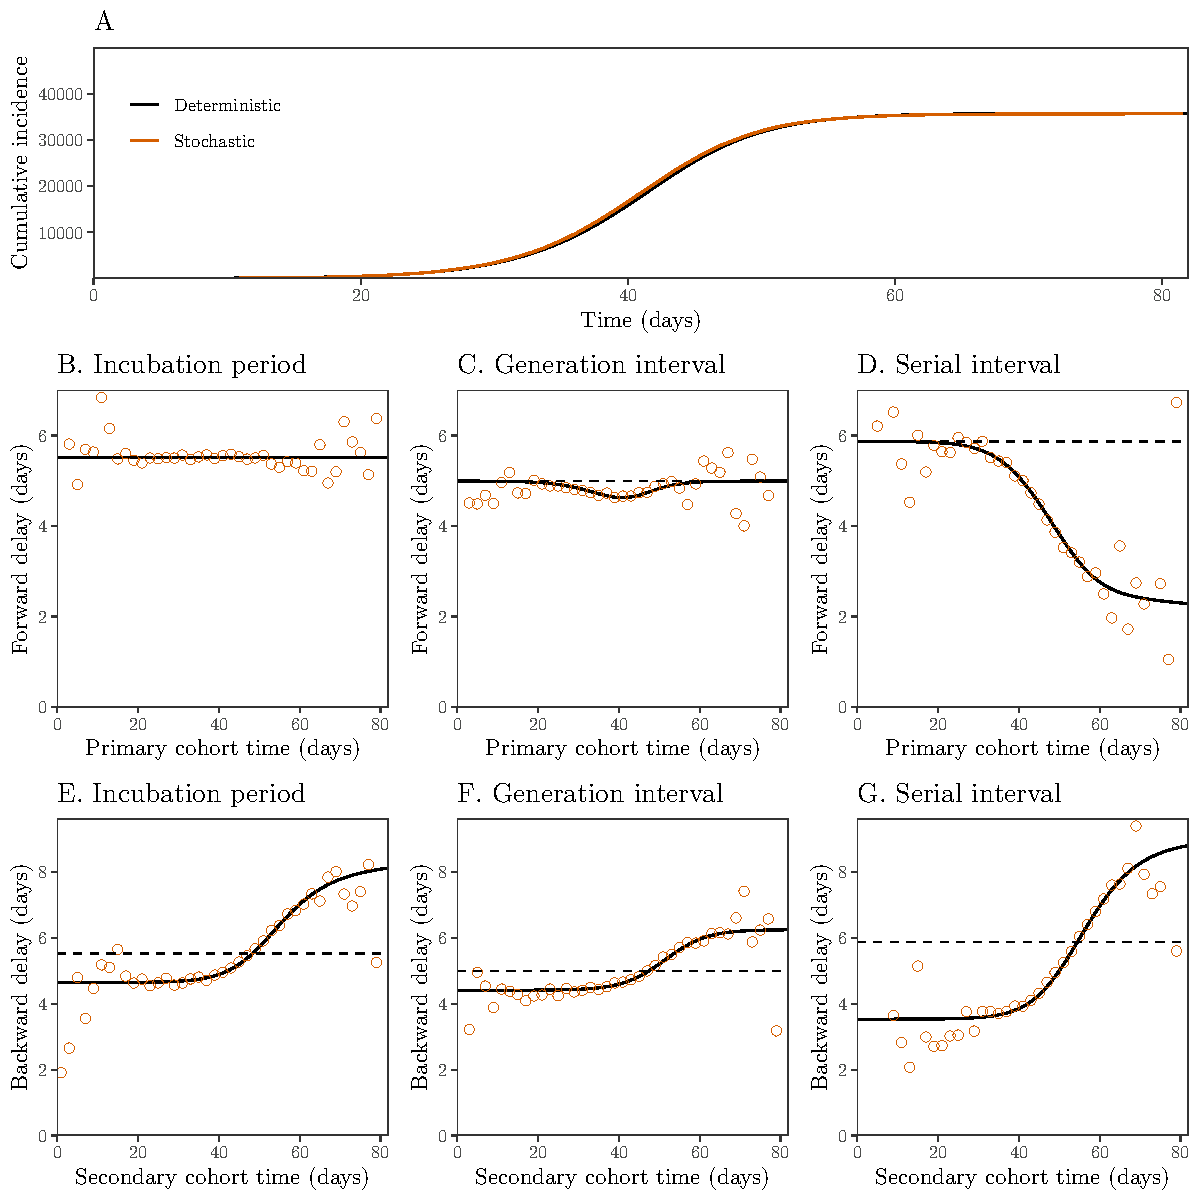
\includegraphics[width=0.95\textwidth]{forward.pdf}
\caption{
\textbf{Epidemiological dynamics and changes in mean forward and backward delay distributions.}
(A) Daily incidence over time.
(B--D) Changes in the mean forward incubation period, generation interval, and serial interval.
(E--G) Changes in the mean backward incubation period, generation interval, and serial interval.
Black \DIFaddbeginFL \DIFaddFL{(A) and colored (B--G) }\DIFaddendFL lines represent the results of a deterministic simulation.
\DIFdelbeginFL \DIFdelFL{Orange }\DIFdelendFL \DIFaddbeginFL \DIFaddFL{Gray }\DIFaddendFL lines (A) represent the results of 10 stochastic simulations.
\DIFdelbeginFL \DIFdelFL{Orange }\DIFdelendFL \DIFaddbeginFL \DIFaddFL{Colored }\DIFaddendFL points (B-G) represent the average of 10 stochastic simulations.
Dashed lines represent the mean initial forward delay.
\DIFaddbeginFL \DIFaddFL{Forward and backward delays are colored according to \fref{diagram}.
In order to remove possible transient dynamics (e.g., left-censoring of time delays and initial stochasticity due to low number of infections), we set $t=0$ to the first time point when daily incidence is greater than 100.
}\DIFaddendFL Intrinsic incubation periods and intrinsic \DIFdelbeginFL \DIFdelFL{generation-intervals }\DIFdelendFL \DIFaddbeginFL \DIFaddFL{generation intervals }\DIFaddendFL are assumed to be independent of each other \DIFaddbeginFL \DIFaddFL{for simplicity}\DIFaddendFL . See \DIFaddbeginFL \DIFaddFL{Supplementary Materials for simulations with correlated incubation periods and generation intervals.
See }\DIFaddendFL Table 1 for parameter values.
}
\label{fig:epi}
\end{center}
\end{figure}

\DIFaddbegin \subsection{\DIFadd{Realized serial-interval distributions during an ongoing epidemic}}

\DIFaddend The initial forward serial-interval distribution captures the exponential growth phase of an epidemic.
We \DIFaddbegin \DIFadd{now }\DIFaddend explore how forward and backward serial intervals can vary over the course of an epidemic using deterministic and stochastic simulations based on the renewal equations (see Supplementary Materials) using parameters in Table 1;
we further assume $\Ro=2.5$ \DIFaddbegin \DIFadd{to reflect the transmission dynamics of COVID-19 in China \mbox{%DIFAUXCMD
\citep{doi:10.1098/rsif.2020.0144}}\hspace{0pt}%DIFAUXCMD
}\DIFaddend .
While the forward serial-interval distribution is our primary focus, understanding the differences between the forward and the backward distributions is important because the observed intervals during an ongoing epidemic are often the backward ones:
we typically identify infected individuals and ask when and by whom they were infected.
Similarly, when we are estimating the incubation period of an individual, we typically observe their symptom onset date and try to estimate when they were infected (e.g., \cite{backer2020incubation}).

\fref{epi} shows the epidemiological dynamics (A) together with the mean forward (B--D) and the mean backward (E--G) delay distributions of a deterministic model based on the renewal equation (\eref{renewal}) and of the corresponding stochastic realizations based on individual-based simulations.
The mean forward incubation period remains constant throughout an epidemic by assumption (\fref{epi}B).
The mean forward generation interval decreases slightly when incidence is high, which is when the susceptible population declines rapidly (\fref{epi}C; \cite{kenah2008generation, champredon2015intrinsic}).
In contrast, the mean forward serial interval decreases over time (\fref{epi}D).

The forward serial-interval distributions depend on distributions of three intervals
(\fref{diagram}\DIFaddbegin \DIFadd{B}\DIFaddend ): (i) the backward incubation period, (ii) the forward generation interval, and (iii) the forward incubation period.
In these simulations, both forward incubation period (\fref{epi}B) and generation-interval (\fref{epi}C) distributions remain roughly constant;
therefore, changes in the forward serial-interval distributions (\fref{epi}D) are predominantly driven by changes in the backward incubation period distribution, whose mean increases over time as the growth rate of disease incidence slows \DIFdelbegin \DIFdel{, then becomes negative}\DIFdelend \DIFaddbegin \DIFadd{and then reverses}\DIFaddend .
In general, relative contributions of the three distributions depend on their shapes, correlations between intrinsic incubation periods and generation intervals, and overall epidemiological dynamics.

We see similar qualitative patterns in all three backward delays (\fref{epi}E--G; \eref{backward}), because they are predominantly driven by the rate of change in incidence, which in turn affects relative cohort sizes.
When incidence is increasing, individuals are more likely to have been infected recently\DIFdelbegin \DIFdel{and therefore, }\DIFdelend \DIFaddbegin \DIFadd{, and therefore }\DIFaddend we are more likely to observe shorter intervals (\eref{backexp}).
Similarly, when incidence decreases, we are more likely to observe longer intervals.
Neglecting these changes \DIFdelbegin \DIFdel{in the backward distributions will necessarily }\DIFdelend \DIFaddbegin \DIFadd{will }\DIFaddend bias the inference of \DIFdelbegin \DIFdel{the }\DIFdelend intrinsic distributions from \DIFdelbegin \DIFdel{the }\DIFdelend observed distributions.

\subsection{Observed serial-interval distributions}

\begin{figure}[!ht]
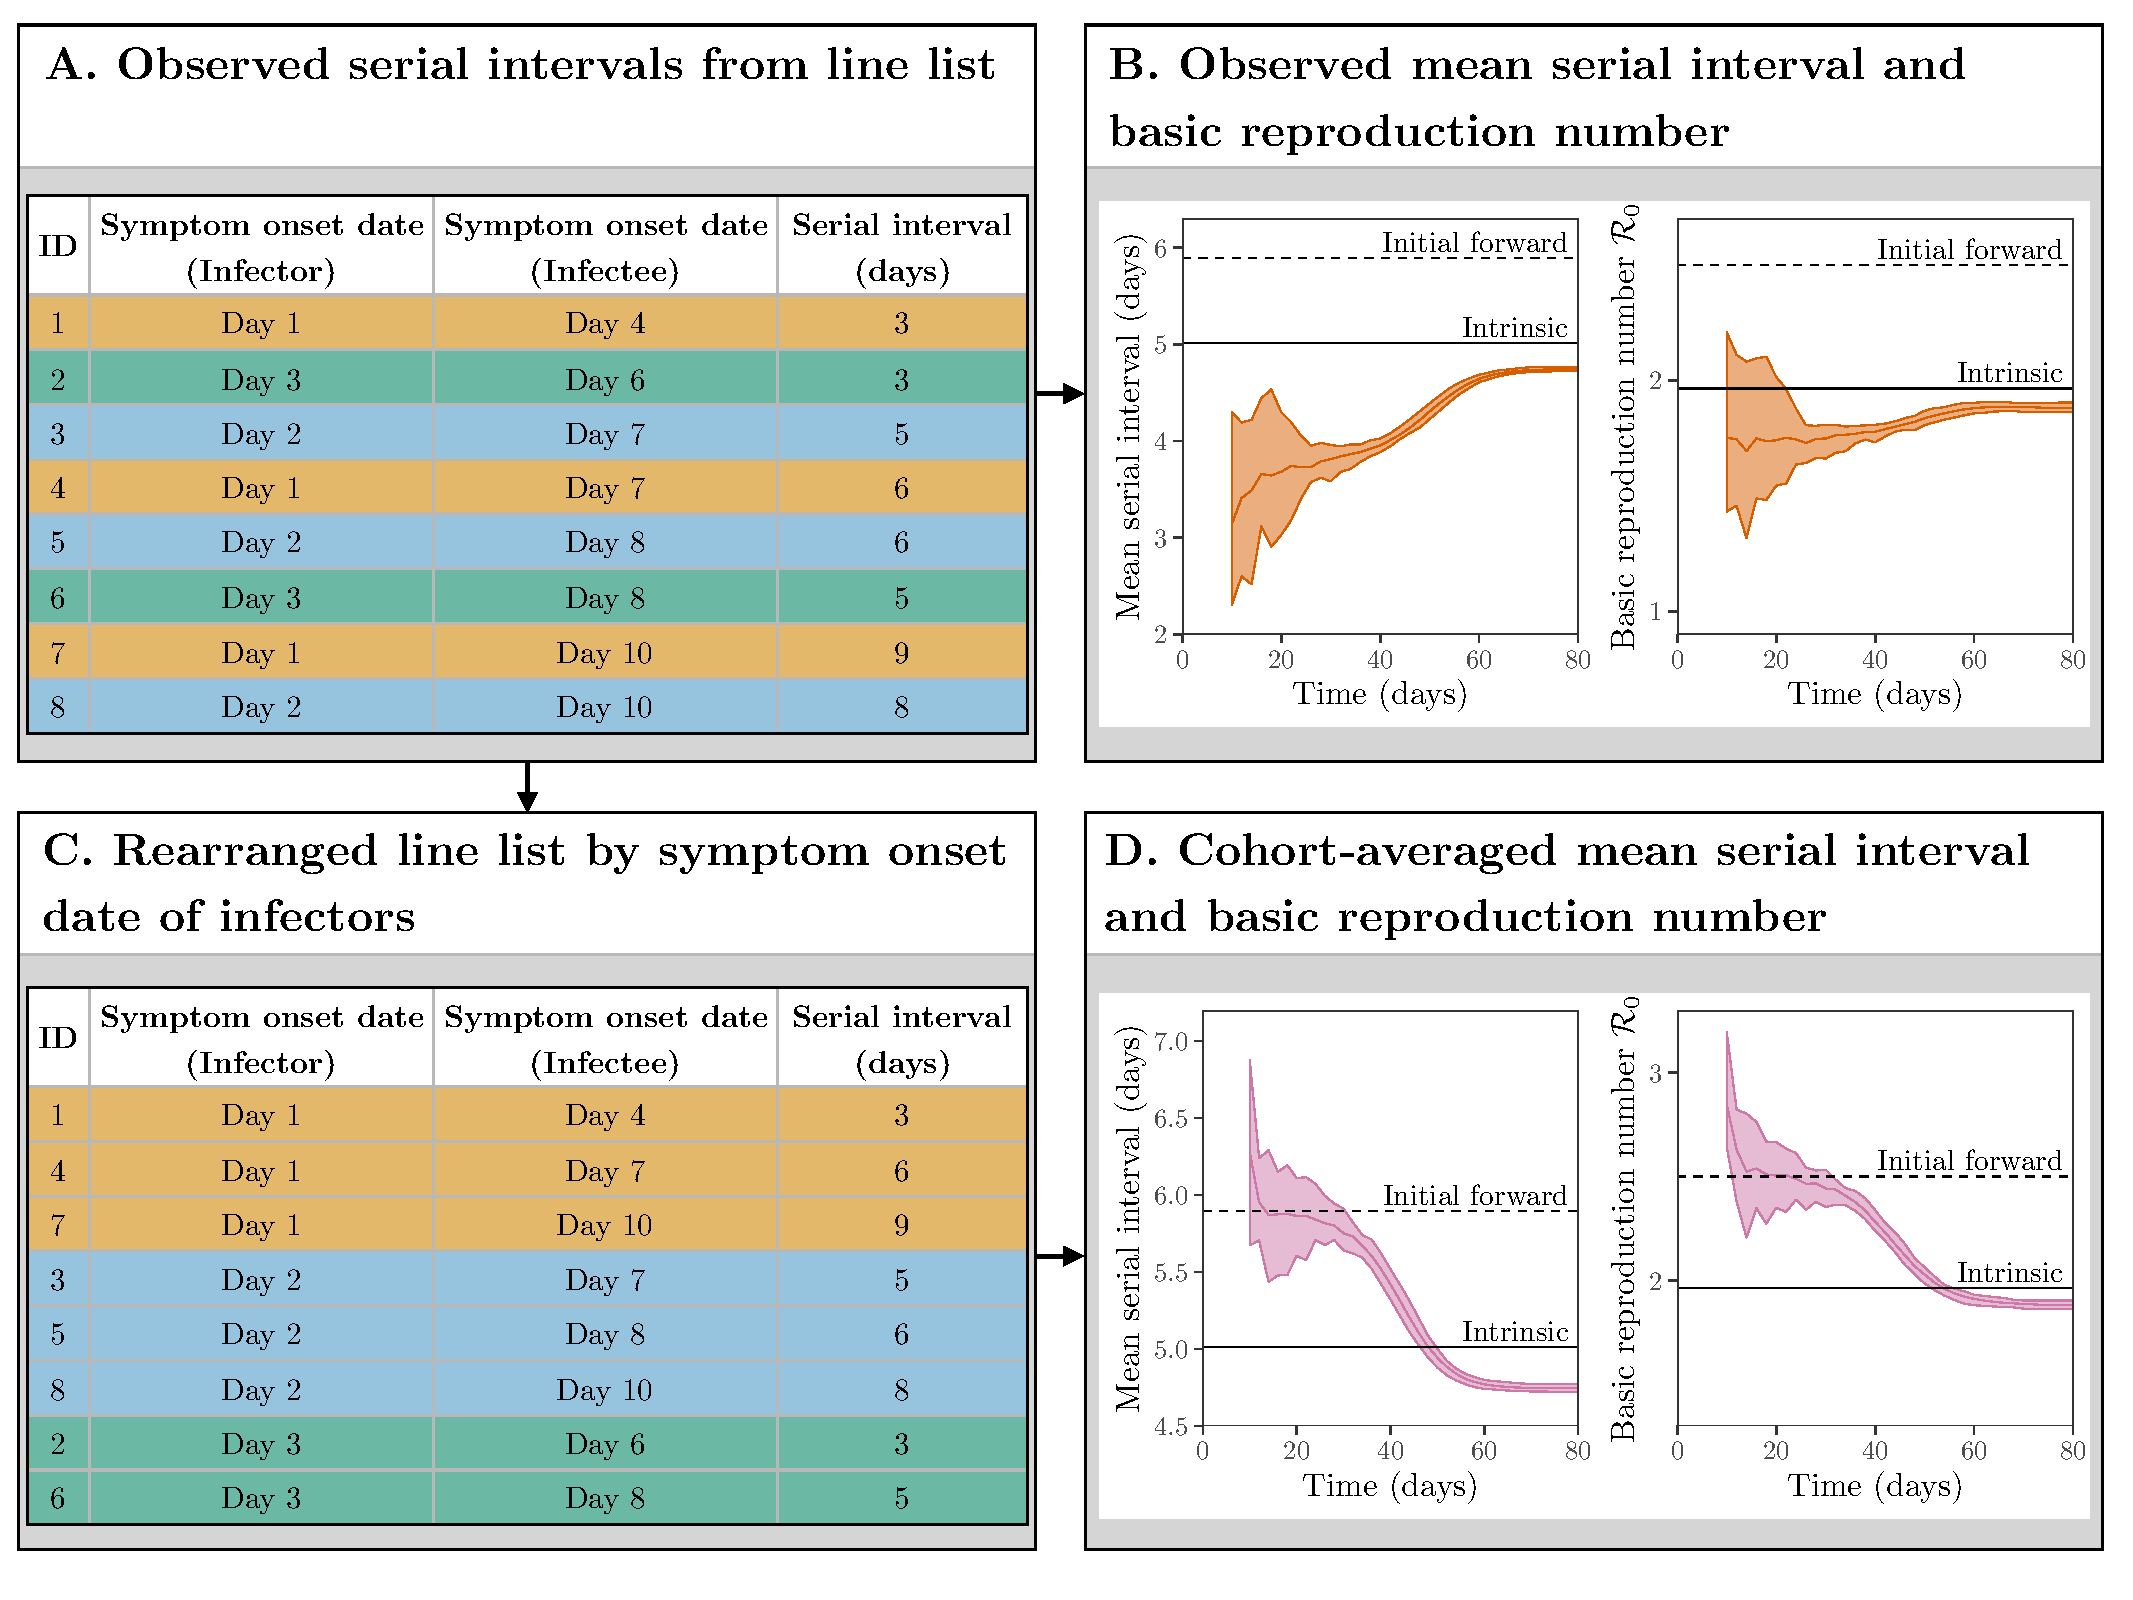
\includegraphics[width=\textwidth]{diagram.pdf}
\caption{
\textbf{Estimating the reproduction number from the observed serial intervals.}
(A) Schematic representation of line list data collected during an epidemic.
(B) Estimates of \Ro based on all observed serial intervals completed by a given time.
(C) Schematic representation of line list data rearranged by symptom onset date of infectors.
(D) Estimates of \Ro based on all observed serial intervals started by a given time. 
Black dashed lines represent the mean initial forward serial interval and \Ro.
Black solid lines represent the mean intrinsic serial interval and \Rintrinsic.
Colored solid lines represent the mean estimates of \Ro across 10 stochastic simulations.
Colored ribbons represent the range of estimates of \Ro across 10 stochastic simulations.
}
\label{fig:obsrR}
\end{figure}

Now, we turn to \DIFaddbegin \DIFadd{practical }\DIFaddend issues of estimating the reproduction number from the observed serial-interval data during on ongoing epidemic.
In order to have an unbiased estimate of the basic reproduction number, we need to estimate the initial forward serial-interval distribution --- i.e., \DIFdelbegin \DIFdel{estimate }\DIFdelend \DIFaddbegin \DIFadd{serial intervals }\DIFaddend based on cohorts of infectors who share the same symptom onset time, at the early stage of the epidemic.
However, researchers typically use all available information to estimate epidemiological parameters \DIFdelbegin \DIFdel{;
in particular, }\DIFdelend \DIFaddbegin \DIFadd{(e.g., aggregating all serial intervals observed until certain time of an epidemic).
For example, }\DIFaddend \cite{thompson2019improved} recently suggested that up-to-date serial-interval data are necessary to accurately estimate the reproduction number.
We explore the consequences of neglecting changes in the realized serial-interval distribution on estimates of the basic reproduction number.

When an epidemic is ongoing, the observed serial intervals are subject to right-censoring because we cannot observe a serial interval if either an infector or an infectee has not yet developed symptoms\DIFdelbegin \DIFdel{;
for }\DIFdelend \DIFaddbegin \DIFadd{.
For }\DIFaddend example, if we were to measure serial intervals on Day 8 as in \fref{obsrR}A, we will only be able to observe the first 6 events (ID 1--6).
\fref{obsrR}B demonstrates how the effect of right-censoring in the observed serial intervals translates to the underestimation of the basic reproduction number \Ro in our stochastic simulations (assuming $\Ro = 2.5$ as in \fref{epi}).
Notably, even if we could observe \DIFdelbegin \DIFdel{, and average, }\DIFdelend \DIFaddbegin \DIFadd{and aggregate }\DIFaddend \emph{all} serial intervals across all transmission pairs after the epidemic has ended, we would still underestimate the initial mean forward serial interval (and therefore \Ro), likely by a large amount\DIFdelbegin \DIFdel{, because the }\DIFdelend \DIFaddbegin \DIFadd{. 
The }\DIFaddend observed serial-interval distribution converges to the intrinsic serial-interval distribution \DIFdelbegin \DIFdel{;
in }\DIFdelend \DIFaddbegin \DIFadd{as the incubation periods and generation intervals will no longer be subject to backward biases.
In }\DIFaddend fact, we would even underestimate the intrinsic value slightly due to contraction of the forward generation-interval distribution during the susceptible depletion phase (\fref{epi}C).
\DIFaddbegin \DIFadd{Therefore, aggregated distributions of serial intervals that have been collected throughout different periods of an epidemic must be interpreted with care.
}\DIFaddend 

Here, we provide a heuristic way of assessing potential biases in the estimate of the mean initial forward serial interval and therefore \Ro retrospectively.
We can rearrange the line list and group observed serial intervals based on the symptom onset date of infectors (\fref{obsrR}C)\DIFaddbegin \DIFadd{---as we showed earlier, serial intervals that share the same symptom onset date of a primary case give us the forward serial-interval distribution}\DIFaddend .
Then, we can compare how \DIFdelbegin \DIFdel{estimates of the mean serial interval }\DIFdelend \DIFaddbegin \DIFadd{the shape of the serial-interval distribution (particularly its mean) }\DIFaddend as well as \DIFaddbegin \DIFadd{the estimate of }\DIFaddend \Ro change as we incorporate more recent cohorts into the analysis\DIFdelbegin \DIFdel{;
}\DIFdelend \DIFaddbegin \DIFadd{:
}\DIFaddend that is, we analyze observed serial intervals from infectors who became symptomatic before time $t$ and evaluate how the estimates change as we increase $t$.
This approach is analogous to averaging over a set of forward intervals, just as using all information up to a certain time is analogous to averaging over a set of backward intervals (\fref{obsrR}D)\DIFaddbegin \DIFadd{;
the major difference is that we we focus on serial intervals that begin in a certain period, rather than those that end in a certain period}\DIFaddend .
During the exponential growth phase, the estimates of the mean serial interval and \Ro are consistent with the true value (see `initial forward' in \fref{obsrR}B,D);
adding more data allows us to make more precise inference during this period.
However, the cohort-averaged estimates decrease rapidly soon after the exponential growth period, reflecting changes in the forward serial-interval distributions.
This approach allows us to detect dynamical changes in the forward serial-interval distributions and their effect on the estimates of \Ro.

\subsection{Applications to the COVID-19 pandemic}

\begin{figure}[!th]
\DIFdelbeginFL %DIFDELCMD < 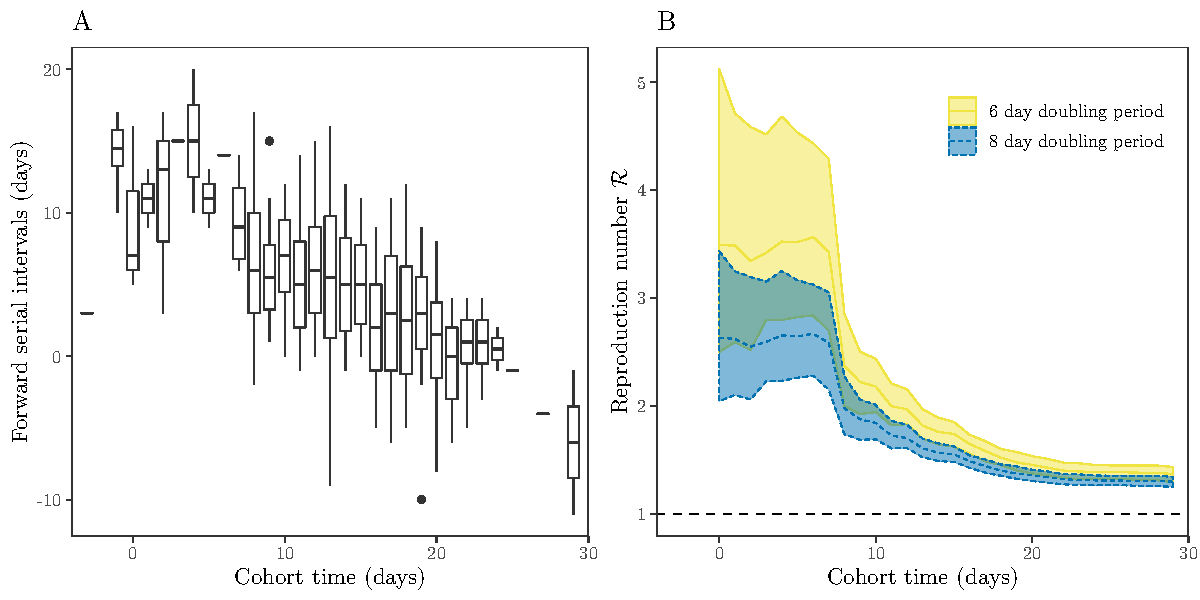
\includegraphics[width=\textwidth]{serial_analysis.pdf}
%DIFDELCMD < %%%
\DIFdelendFL \DIFaddbeginFL \begin{center}
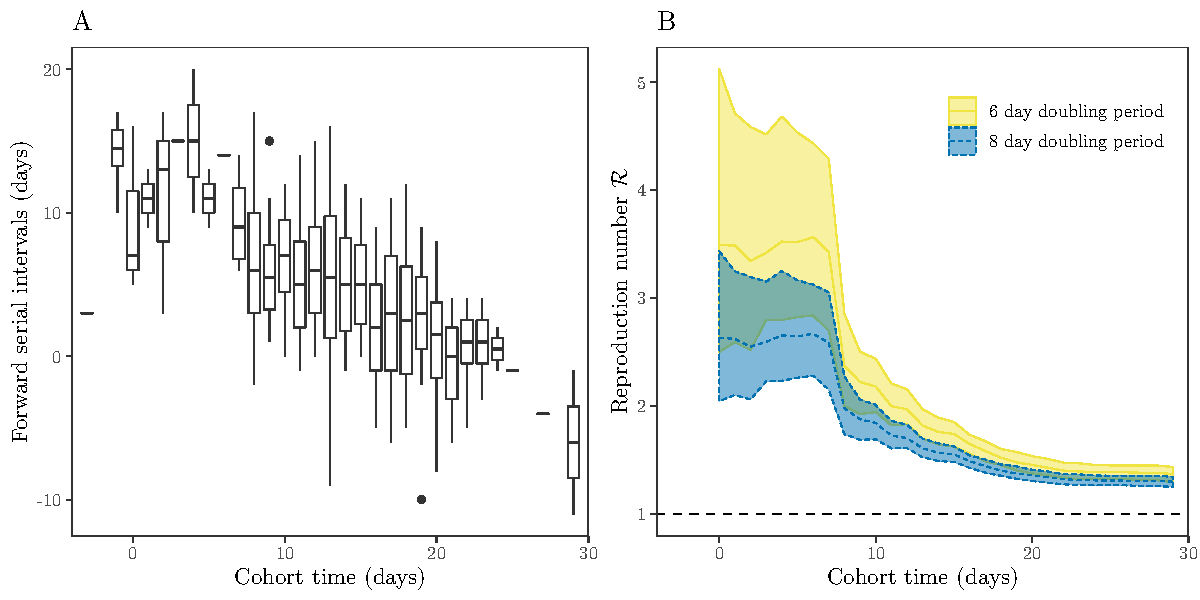
\includegraphics[width=0.85\textwidth]{serial_analysis.pdf}
\DIFaddendFL \caption{
\textbf{Observed serial intervals of COVID-19 and cohort-averaged estimates of \RR.}
(\DIFdelbeginFL \DIFdelFL{A--B}\DIFdelendFL \DIFaddbeginFL \DIFaddFL{A}\DIFaddendFL ) \DIFaddbeginFL \DIFaddFL{Symptom onset dates of all individuals within 468 transmission pairs included in the contact tracing data.
(B--C) }\DIFaddendFL forward and backward serial intervals over time.
\DIFaddbeginFL \DIFaddFL{Serial interval data have been grouped based on the symptom onset dates of primary (B) and secondary (C) cases.
}\DIFaddendFL Points represent the means. 
Vertical error bars represent the 95\% equi-tailed quantiles.
Solid lines represent the estimated locally estimated scatterplot smoothing (LOESS) fits.
The dashed line represents the maximum and minimum observable delays across the range of reported symptom onset dates.
(\DIFdelbeginFL \DIFdelFL{C}\DIFdelendFL \DIFaddbeginFL \DIFaddFL{D}\DIFaddendFL ) Cohort-averaged estimates of \Ro assuming doubling period of 6 and 8 days \citep{li2020early, wu2020nowcasting}.
Ribbons represent the associated 95\% bootstrap confidence intervals.
The data were taken from Supplementary Materials of \cite{du2020serial}.
}
\label{fig:du}
\DIFaddbeginFL \end{center}
\DIFaddendFL \end{figure}

Finally, we re-analyze serial intervals of COVID-19 collected by \cite{du2020serial} from mainland China, outside Hubei province, based on \DIFaddbegin \DIFadd{468 }\DIFaddend transmission events reported between January 21--February 8, \DIFdelbegin \DIFdel{2020;
}\DIFdelend \DIFaddbegin \DIFadd{2020.
}\DIFaddend \cite{du2020serial} estimated the mean serial interval of 3.96 days (95\% CI 3.53–4.39 days) and \Ro of 1.32 (95\% CI 1.16–1.48).
\fref{du}A shows \DIFaddbegin \DIFadd{the distribution of symptom onset dates of all individuals within 468 transmission pairs (consisting a total of 752 unique individuals), resembling a COVID-19 epidemic curve in China (cf. Fig. 1 in \mbox{%DIFAUXCMD
\cite{pan2020jama}}\hspace{0pt}%DIFAUXCMD
).
In order to quantify changes in serial intervals, we group them by the symptom onset dates of the primary (\fref{du}B) and secondary (\fref{du}C) cases---corresponding to forward and backward serial-interval distributions, respectively---and compute their mean and 95\% quantiles.
\fref{du}B shows }\DIFaddend that the mean forward serial interval decreases over time.
While the decrease is likely to be affected by the right-censoring (indicated by the closeness between the quantiles of the observed serial intervals and maximum observable serial intervals), the increase in the proportion of negative serial intervals indicates changes in the forward serial-interval distribution;
this proportion is unlikely to be affected by left-censoring (based on the gap between the quantiles of the observed serial intervals and minimum observable serial intervals).
The decrease in the mean forward serial interval was probably driven by interventions against spread.
Interventions during this time period both decreased (and then reversed) the growth rate of COVID-19 cases --- thus increasing the backward incubation period --- and also reduced generation intervals, by preventing infections once cases were identified.
Both of these would have acted to reduce the forward serial interval.
\fref{du}\DIFdelbegin \DIFdel{B }\DIFdelend \DIFaddbegin \DIFadd{C }\DIFaddend shows that the mean backward serial interval increased over time, \DIFaddbegin \DIFadd{also }\DIFaddend likely driven directly by the decrease in COVID-19 \DIFdelbegin \DIFdel{cases}\DIFdelend \DIFaddbegin \DIFadd{infections}\DIFaddend .

While the qualitative changes in the mean forward and backward serial interval are consistent with our earlier simulations (\fref{epi}), the initial mean forward serial interval (\fref{du}\DIFdelbegin \DIFdel{A}\DIFdelend \DIFaddbegin \DIFadd{B}\DIFaddend ) appears to be larger than what we calculated based on previously estimated incubation period and generation-interval distributions (\fref{rR}C).
\DIFdelbegin \DIFdel{These }\DIFdelend \DIFaddbegin \DIFadd{This difference }\DIFaddend may imply that the incubation period and generation interval (Table 1) were underestimated, as neither study explicitly accounted for the fact that the observed intervals were drawn from the backward distributions and were likely to have been censored.

\fref{du}\DIFdelbegin \DIFdel{C }\DIFdelend \DIFaddbegin \DIFadd{D }\DIFaddend shows the cohort-averaged estimates of \Ro, which remain roughly constant until day \DIFdelbegin \DIFdel{7 }\DIFdelend \DIFaddbegin \DIFadd{January 17th }\DIFaddend and suddenly decreases;
this sudden decrease is due \DIFaddbegin \DIFadd{to }\DIFaddend changes in the forward serial intervals consistent with the dynamics seen in our simulations (\fref{obsrR}).
The cohort-averaged estimates of \Ro based on the early forward serial intervals are also consistent with previous estimates of \Ro of the COVID-19 epidemic in China \DIFdelbegin \DIFdel{\mbox{%DIFAUXCMD
\citep{majumder2020early, park2020reconciling}}\hspace{0pt}%DIFAUXCMD
}\DIFdelend \DIFaddbegin \DIFadd{\mbox{%DIFAUXCMD
\citep{majumder2020early, doi:10.1098/rsif.2020.0144}}\hspace{0pt}%DIFAUXCMD
}\DIFaddend :
$\Ro = 2.6$ (95\% CI: 2.2--3.1) and $\Ro = 3.4$ (95\% CI: 2.7 -- 4.3) based on \DIFaddbegin \DIFadd{a doubling period of }\DIFaddend 8 \DIFdelbegin \DIFdel{and }\DIFdelend \DIFaddbegin \DIFadd{or }\DIFaddend 6 \DIFdelbegin \DIFdel{doubling periods}\DIFdelend \DIFaddbegin \DIFadd{days}\DIFaddend , respectively, using serial-interval data from infectors who developed symptoms by \DIFdelbegin \DIFdel{day 7.
}\DIFdelend \DIFaddbegin \DIFadd{January 17th.
}\DIFaddend These early cohort-averaged estimates of \Ro are unlikely to be affected by the right-censoring as we expect the degree of right-censoring to be low (\fref{du}A).
Therefore, the \DIFaddbegin \DIFadd{original }\DIFaddend \Ro estimate of 1.32 (95\% CI 1.16\DIFaddbegin \DIFadd{-}\DIFaddend –1.48), which neglects the changes in the forward serial-interval distribution, \DIFdelbegin \DIFdel{is likely to be an underestimate}\DIFdelend \DIFaddbegin \DIFadd{underestimates }\Ro \DIFadd{by a factor of 2.0--2.6}\DIFaddend .
This example demonstrates the danger of using the observed serial intervals to calculate the reproduction number without organizing serial intervals into cohorts.

\section{Discussion}

Generation and serial intervals determine the time scale of disease transmission, and are therefore critical to dynamical modeling of infectious outbreaks.
\DIFdelbegin \DIFdel{Here, we show }\DIFdelend \DIFaddbegin \DIFadd{We have shown }\DIFaddend that the initial \emph{forward} serial-interval distribution --- measured \DIFaddbegin \DIFadd{from the cohort of infectors who developed symptoms }\DIFaddend during the exponential growth phase of an epidemic --- provides the correct link between the exponential growth rate $r$ and the \DIFaddbegin \DIFadd{initial }\DIFaddend reproduction number \RR.
In general, the forward serial-interval distributions will not match the intrinsic \DIFdelbegin \DIFdel{or the backward }\DIFdelend serial-interval \DIFdelbegin \DIFdel{distributions}\DIFdelend \DIFaddbegin \DIFadd{distribution (which has the same mean as the intrinsic generation-interval distribution) because the incubation period of the infectors (conditional on their symptom onset date of the infector) will be subject to backward biases}\DIFaddend .
In particular, the mean forward serial interval can decrease over time \DIFdelbegin \DIFdel{due to epidemic dynamics}\DIFdelend \DIFaddbegin \DIFadd{for COVID-19 as individuals who develop symptoms later in an epidemic are more likely to have longer incubation periods, and therefore have greater opportunity to transmit presymptomatically}\DIFaddend .
Failing to account for these effects can result in underestimation of \DIFaddbegin \DIFadd{initial }\DIFaddend \RR.

\DIFdelbegin \DIFdel{Our study underlines the importance of carefully defining measured epidemiological time distributions. Previous studies have shown that it matters whether generation
intervals are measured forward or backward \mbox{%DIFAUXCMD
\citep{nishiura2010time,champredon2015intrinsic,britton2019estimation}}\hspace{0pt}%DIFAUXCMD
;
we generalize these ideas and show that they apply to other epidemiological distributions.
Changes in the backward delaydistributions due to changing cohort sizes are expected to be a pervasive feature of outbreak dynamics.
Recent analyses of }\DIFdelend \DIFaddbegin \DIFadd{Recently, \mbox{%DIFAUXCMD
\cite{ali2020serial} }\hspace{0pt}%DIFAUXCMD
also showed that forward serial intervals of }\DIFaddend COVID-19 \DIFdelbegin \DIFdel{epidemics have attempted to reconstruct epidemic time series from by using time-independent delay distributions from infection or symptom onset to reporting (e.g., \mbox{%DIFAUXCMD
\cite{tempvar, park2020potential,scire2020reproductive,shim2020transmission}}\hspace{0pt}%DIFAUXCMD
);
these studies effectively assume constant backward delay distributions.
Although such approaches may be able to roughly match the time scale }\DIFdelend \DIFaddbegin \DIFadd{decreased through time in China. They grouped serial intervals by the symptom onset date of infectors across 14-day periods and found that the mean forward serial interval decreased from 7.8 days to 2.6 days.
While they attributed the decrease in serial intervals to reduction of the isolation delay, their regression analysis showed that isolation delays explain only 51.5\% of the variation in serial intervals (they could explain up to 72\% of the variance by including other intervention measures).
Our framework provides an explanation for the remaining variation: changes in the backward incubation period during the decreasing phase }\DIFaddend of an epidemic \DIFdelbegin \DIFdel{, we show here that they are subject to bias.
Dynamical approaches that model explicitly model incidence as well as reporting delays (e.
g., \mbox{%DIFAUXCMD
\cite{flaxman2020estimating}}\hspace{0pt}%DIFAUXCMD
) can avoid this problem, but at the cost of more complexity in estimation. There is a need for simple methods that can complement more explicit approaches of addressing this problem}\DIFdelend \DIFaddbegin \DIFadd{act to further shorten serial intervals due to increased amount of presymptomatic transmission (even in the absence of nonpharmaceutical interventions).
Isolation delays and other intervention measures affect the amount of onward transmission, and therefore the distribution of realized (forward) generation intervals.
They therefore are not expected to explain all the variation in forward serial intervals, since these additionally depend on both the backward incubation period of the infector and the forward incubation period of the infectee (\fref{diagram}B)}\DIFaddend .

\DIFdelbegin \DIFdel{While our }\DIFdelend \DIFaddbegin \DIFadd{Our }\DIFaddend results support the use of serial-interval distributions for calculating \DIFaddbegin \DIFadd{the }\DIFaddend \RR \DIFdelbegin \DIFdel{, 
}\DIFdelend \DIFaddbegin \DIFadd{during the exponential growth phase,  
but }\DIFaddend they also reveal gaps in current practices in incorporating serial-interval distributions into outbreak analyses.
\DIFaddbegin \DIFadd{For example, }\DIFaddend \cite{thompson2019improved} recently emphasized the importance of using up-to-date serial-interval data for accurate estimation of time-varying reproduction numbers.
\DIFdelbegin \DIFdel{We show here, however, that if changes }\DIFdelend \DIFaddbegin \DIFadd{However, our results show that if observational biases in }\DIFaddend the forward serial interval through time are not accounted for, using up-to-date serial-interval data can \DIFdelbegin \DIFdel{, in fact, }\DIFdelend \DIFaddbegin \DIFadd{actually }\DIFaddend exacerbate the underestimation of \DIFdelbegin \DIFdel{initial }\DIFdelend \RR \DIFaddbegin \DIFadd{in the initial growth phase of an outbreak}\DIFaddend .
Future studies should explore how neglecting changes in the forward serial-interval distribution can affect the estimates of \RR beyond the exponential growth phase\DIFaddbegin \DIFadd{, }\DIFaddend and potentially re-assess existing estimates of \RR.
\DIFdelbegin %DIFDELCMD < 

%DIFDELCMD < %%%
\DIFdel{Many studies have already estimated the (time-varying) reproduction numbers for COVID-19 epidemics using aggregated serial-interval data (e.g., \mbox{%DIFAUXCMD
\cite{tempvar,du2020serial,pan2020jama,zhang2020evolving}}\hspace{0pt}%DIFAUXCMD
);
these studies should also re-assess whether they appropriately considered the }\emph{\DIFdel{forward}} %DIFAUXCMD
\DIFdel{serial interval.
Forward serial-interval distributions are also likely to vary across countries.
We }\DIFdelend \DIFaddbegin \DIFadd{We also }\DIFaddend suggest that modelers should aim to characterize spatiotemporal variation in forward serial-interval distributions\DIFdelbegin \DIFdel{and understand their changes over time}\DIFdelend .
These modeling approaches should be coupled with epidemiological investigation through contact tracing. 
Going forward, an additional advantage of early, intensive contact tracing of emerging diseases is that \DIFdelbegin \DIFdel{this is the best way }\DIFdelend \DIFaddbegin \DIFadd{it provides the best information }\DIFaddend to characterize the initial forward serial-interval distribution.

Our study \DIFdelbegin \DIFdel{also }\DIFdelend underlines the fact that the serial-interval distribution depends not only on the generation-interval and incubation-period distributions, but also on \DIFdelbegin \DIFdel{their intrinsic correlations.
This implies that not considering this correlation can bias the estimates of the intrinsic generation-interval distribution from the }\DIFdelend \DIFaddbegin \DIFadd{the correlation between their duration in a given individual.
Here, we use a bivariate lognormal distribution to capture these correlations phenomenologically and to show that realized serial intervals can decrease over time in the context of COVID-19.
Although their true correlation will depend on viral load dynamics, we expect our conclusions about decreasing serial intervals of COVID-19 to be robust, as individuals with longer incubation periods will generally have a longer time window to transmit before symptom onset.
In general, the impact of increasing backward incubation periods on the forward serial intervals are likely to be disease-specific---for example, we show in Supplementary Materials that the initial forward }\DIFaddend serial-interval distribution \DIFdelbegin \DIFdel{.
Previous studies that tried to estimate the generation-interval distributions from }\DIFdelend \DIFaddbegin \DIFadd{can be equivalent to }\DIFaddend the \DIFdelbegin \DIFdel{observed serial intervals often ignored the dynamical differences between the realized incubation periodsof infectors (backward-looking) and those of infectees (forward looking) (e.
g.
, \mbox{%DIFAUXCMD
\cite{klinkenberg2011correlation, ganyani2020estimating}}\hspace{0pt}%DIFAUXCMD
).
Better statistical tools for teasing apart the }\DIFdelend intrinsic \DIFdelbegin \DIFdel{generation-interval distributionsfrom the observed serial intervals are needed.
}\DIFdelend \DIFaddbegin \DIFadd{generation-interval distribution, regardless of the growth rate $r$, due to independence between the incubation period and time from symptom onset to transmission and the lack of presymptomatic transmission.
Future studies trying to interpret realized serial intervals should consider carefully the joint distribution between the generation intervals and incubation periods.
}\DIFaddend 

\DIFaddbegin \DIFadd{In closing, we lay out a few practical principles for analyzing and interpreting serial-interval data.
First, serial intervals should be cohorted based on the symptom onset date of the infector (and not of the infectee) whenever possible.
Previous studies have often regarded serial intervals as an intrinsic quantity, having the same mean as the intrinsic generation interval \mbox{%DIFAUXCMD
\citep{svensson2007note,klinkenberg2011correlation,champredon2018equivalence, britton2019estimation}}\hspace{0pt}%DIFAUXCMD
, but the distribution (and the mean) of observed serial intervals differs from this expectation, and changes through time due to epidemic dynamics.
Second, aggregating serial intervals across different cohorts and epidemic periods should be avoided because the realized serial-interval distribution can be subject to different censoring and epidemiological biases:
Even when }\emph{\DIFadd{all}} \DIFadd{realized serial intervals can be observed throughout an unmitigated epidemic, we do not obtain the intrinsic serial interval distribution due to susceptible depletion (\fref{obsrR}).
Third, applying serial-interval information across epidemics of a given disease should be done with care, because serial intervals are epidemic-specific, rather than disease-specific.
Finally, serial-interval data should be accompanied by a trajectory of the epidemic curve, whenever possible, to provide epidemiological context.
In practice, these recommendations will sometimes be hard to follow, due to limited data about serial intervals, but these issues should be kept in mind when interpreting serial-interval data to inform transmission dynamics.
}

\DIFadd{More broadly, our study underlines the importance of carefully defining measured epidemiological time distributions. 
Previous studies have shown the importance of forward vs. backward
measurement of generation intervals \mbox{%DIFAUXCMD
\citep{nishiura2010time,champredon2015intrinsic,britton2019estimation}}\hspace{0pt}%DIFAUXCMD
;
we generalize these ideas and show that they apply to other epidemiological distributions.
Some studies during the early phases of the COVID-19 epidemics have tried to correct for the backward biases \mbox{%DIFAUXCMD
\citep{verity2020estimates}}\hspace{0pt}%DIFAUXCMD
, but changes in the backward delay distributions due to changing cohort sizes are expected to be a pervasive feature of outbreak dynamics.
Cohorting epidemiological delays by the primary event time can help avoid backward biases (although censoring biases can still exist) as well as detect potential changes in the distribution.
}

\DIFaddend Here, we assume that all individuals develop symptoms and that the entire transmission process, including all relevant epidemiological delays, is known exactly.
In practice, identifying who infected whom is difficult in general, and asymptomatic and presymptomatic transmission of COVID-19 exacerbates this difficulty \citep{bai2020presumed,he2020temporal,wei2020presymptomatic}.
Biases in the observed serial intervals will necessarily bias the estimates of \RR. 
Furthermore, when one of the individuals \DIFaddbegin \DIFadd{in a transmission pair }\DIFaddend is asymptomatic, there is no symptom-based serial interval\DIFdelbegin \DIFdel{; 
neglecting }\DIFdelend \DIFaddbegin \DIFadd{.
Neglecting }\DIFaddend the time scale \DIFaddbegin \DIFadd{of }\DIFaddend asymptomatic transmission may also bias the estimates of \RR \citep{park2020time}.

\DIFdelbegin \DIFdel{While we focus here on the effect of epidemiological dynamics on serial-interval distributions, other factors, such as intervention strategies, can also affect the generation- and serial-interval distributions.
Individual-level interventions, such as case isolation, and behavioral responses directly affect individuals' ability to transmit and will shorten the forward generation- and serial-intervals.
Population-level interventions, such as social distancing, can squeeze contacts into household and induce clustering, which will in turn shorten the realized generation interval due to local depletion of the susceptible pool within households \mbox{%DIFAUXCMD
\citep{park2019inferring}}\hspace{0pt}%DIFAUXCMD
.
}%DIFDELCMD < 

%DIFDELCMD < %%%
\DIFdelend Despite these limitations, our analysis of serial intervals of COVID-19 from China provides further support for our theoretical framework, demonstrating temporal variation in serial intervals and its effect on the estimates of \RR.
Most existing estimates of the serial-intervals of COVID-19 implicitly or explicitly assume that the serial-interval distributions remain constant throughout the course of an epidemic \citep{du2020serial, he2020temporal, nishiura2020serial,tindale2020transmission,zhao2020estimating,zhang2020evolving}.
Our study provides a rationale for reassessing estimates of
serial-interval distributions---and their use in estimating
\RR---during the COVID-19 pandemic.

\DIFaddbegin \section*{\DIFadd{Data availability}}

\DIFadd{All data and code are stored in a publicly available GitHub repository (}\url{https://github.com/parksw3/serial}\DIFadd{).
}

\DIFaddend \pagebreak

\section{Supplementary Materials}

\subsection{Deterministic simulation}

We simulate the renewal equation model using a discrete-time approximation:
\begin{align}
i(t) &= \Ro S(t-\Delta t) \sum_{m=1}^{\tsub{m}{max}} i(t-m \Delta t) \hat{\gdist}(m \Delta t) \nonumber \\
S(t) &= S(t-\Delta t) - i(t)
\end{align}
where $\hat{\gdist}$ is a discrete-time intrinsic generation-interval distribution that satisfies the following:
\begin{equation}
\hat{\gdist}(m \Delta t) = \frac{\gdist(m \Delta t)}{\sum_{i=1}^\ell \gdist(m \Delta t)}, \quad m=1, \dots, \tsub{m}{max}.
\end{equation}
The continuous-time intrinsic generation-interval distribution is parameterized using a log-normal distribution (Table 1). We define the intrinsic incubation period distribution in a similar manner:
\begin{equation}
\hat{\idist}(m \Delta t) = \frac{\idist(m \Delta t)}{\sum_{i=1}^\ell \idist(m \Delta t)}, \quad m=1, \dots, \tsub{m}{max},
\end{equation}
where its continuous-time analog is also based on a log-normal distribution.
For simplicity, we assume that the forward incubation periods and intrinsic generation intervals are independent:
\begin{equation}
\hat{h}(m \Delta t, n \Delta t) = \hat{\idist}(m \Delta t)\hat{\gdist}(n \Delta t), \quad m,n=1, \dots, \tsub{m}{max}.
\end{equation}
We use $\Delta t = 0.025\,\textrm{days}$ and $\tsub{m}{max}=2001$ for discretization steps.

We initialize the simulation with population size $N$=40,000 as follows:
\begin{align}
i(m \Delta t) &= C \exp(r m \Delta t), \quad m=1, \dots, \tsub{m}{max}\nonumber \\
S(m \Delta t) &= N - \sum_{n=1}^m i(n \Delta t), \quad m=1, \dots, \tsub{m}{max}
\end{align}
where $C$ is chosen such that $\sum_{n=1}^{\tsub{m}{max}} i(m \Delta t)=10$.
These initial conditions allow the model to follow exponential growth from time $\Delta t (\tsub{m}{max} + 1)$ without any transient behaviors.
\DIFdelbegin \DIFdel{Results presented in the main text show simulations beginning from time $\Delta t (\tsub{m}{max} + 1)$.
}\DIFdelend 

\subsection{Stochastic simulation}

We run stochastic simulations of the renewal equation model using an individual-based model on a fully connected network (i.e., homogeneous population) based on the Gillespie algorithm that we developed earlier \DIFdelbegin \DIFdel{\mbox{%DIFAUXCMD
\citep{park2019inferring}}\hspace{0pt}%DIFAUXCMD
}\DIFdelend \DIFaddbegin \DIFadd{\mbox{%DIFAUXCMD
\citep{park2020inferring}}\hspace{0pt}%DIFAUXCMD
}\DIFaddend .
First, we initialize an epidemic with $I(0)$ infected individuals (nodes) in a fully connected network of size $N$. 
For each initially infected individual, we draw number of infectious contacts from a Poisson distribution with the mean of \Ro and the corresponding generation intervals for each contact from a log-normal distribution (Table 1).
Contactees are uniformly sampled from the total population.
All contactees are sorted into event queues based on their infection time.
We update the current time to the infection time of the first person in the queue.
Then, the first person in the queue makes contacts based on the Poisson offspring distribution described earlier and their contactees are added to the sorted queue.
Whenever contactees are added to the sorted queue, we remove all duplicated contacts (but keep the first one) as well as contacts made to individuals that have already been infected.
Simulations continue until there are no more individuals in the queue.
We simulate 10 epidemics with $I(0)=10$ and $N$=40,000.

\subsection{Linking $r$ and \Ro using serial-interval distributions}

The intrinsic generation-interval distribution $\gdist(\tau)$ provides a link between $r$ and \Ro via the Euler-Lotka equation \citep{wallinga2007generation}:
\begin{equation}
\frac{1}{\Ro} = \int_0^\infty \exp(-r\tau) \gdist(\tau) \dtau\,.
\end{equation}
In this section, we prove that the initial forward serial-interval distribution $f_0(\tau)$ also estimates the same \Ro from $r$, except that integral extends to $\tau=-\infty$ rather than beginning at $\tau=0$, because serial intervals can be negative:
\begin{equation}
\frac{1}{\Ro} = \int_{-\infty}^\infty \exp(-r\tau) f_{0}(\tau) \dtau\,.
\label{eq:ptarget}
\end{equation}
Here, the initial forward serial-interval distribution $f_{0}(\tau)$ is defined as:
\begin{equation}
f_{0}(\tau) = \frac{1}{\phi} \int_{-\infty}^{0} \int_{\alpha_1}^{\tau} \exp(r \alpha_1) h(-\alpha_1, \alpha_2 - \alpha_1) \idist(\tau - \alpha_2) \, \mathrm{d}\alpha_2\,\mathrm{d}\alpha_1\,,
\label{eq:fdist}
\end{equation}
where $h$ is the joint probability distribution describing the
intrinsic generation-interval distribution $g$ and the intrinsic
incubation period distribution $\idist$ (see \eref{marginal} in the
main text), and the normalization constant $\phi$ is determined by the
requirement that $\int_{-\infty}^\infty f_{0}(\tau)\,\dtau=1$.

In order to verify \eref{ptarget}, we first rewrite the integral in \eref{fdist} by substituting $-\alpha_1$ for $\alpha_1$, and then changing the order of integration:
\begin{align}
f_{0}(\tau) &= \frac{1}{\phi} \int_0^\infty \int_{-\pinf}^{\tau} \exp(-r\pinf) h(\pinf, \sinf + \pinf) \idist(\tau - \sinf)\, \mathrm{d}\sinf\,\mathrm{d}\pinf\,,\nonumber \\
&= \frac{1}{\phi} \int_{-\infty}^{\tau} \int_{\max{(0,-\sinf)}}^{\infty} \exp(-r\pinf) h(\pinf, \sinf + \pinf)\idist(\tau - \sinf)\,\mathrm{d}\pinf\, \mathrm{d}\sinf\,.
\label{eq:newforward}
\end{align}
To further simplify the expression, we define $z(\sinf)$ as follows:
\begin{equation}
z(\sinf) = \int_{\max{(0,-\sinf)}}^{\infty} \exp(-r\pinf) h(\pinf, \sinf + \pinf) \,\mathrm{d}\pinf\,.
\end{equation}
Substituting $z(\sinf)$ into \eref{newforward} we obtain:
\begin{equation}
f_{0}(\tau) = \frac{1}{\phi} \int_{-\infty}^{\tau} z(\sinf) \idist(\tau - \sinf) \,\mathrm{d}\sinf\,,.
\end{equation}
Writing $\hat{z}$ for a normalized version of $z$,
\begin{equation}\hat{z}(\sinf) = \frac{z(\sinf)}{\int_{-\infty}^\infty z(x) \dx}\,,\end{equation}
we can now express the initial forward serial-interval distribution
$f_0$ as a convolution of $\hat{z}$ and $\idist$:
\begin{equation}
f_{0}(\tau) = \frac{1}{\hat{\phi}} \int_{-\infty}^{\tau} \hat{z}(\sinf) \idist(\tau - \sinf)\, \mathrm{d}\sinf\,,
\end{equation}
where $\hat{\phi} = \phi/\int_{-\infty}^\infty z(x) \dx$.

Since the right hand side of \eref{ptarget} is also a
Laplace transform of $f_0=\hat{z}*\idist$, we can express it as the product
of Laplace transforms of $\hat{z}$ and $\idist$:
\begin{equation}
\int_{-\infty}^\infty \exp(-r\tau) f_{0}(\tau) \mathrm{d} \tau = \int_{-\infty}^\infty \exp(-r\tau) \hat{z}(\tau)\, \mathrm{d} \tau \int_{0}^\infty \exp(-r\tau) \idist(\tau) \dtau\,.
\label{eq:newtarget}
\end{equation}
In order to derive an expression for a Laplace transform of $\hat{z}$, we have to first derive an analytical expression for $\int_{-\infty}^\infty z(x) \dx$. By changing the order of integration, we have:
\begin{align}
\int_{-\infty}^\infty z(\sinf) \mathrm{d}\sinf &= \int_{-\infty}^\infty \int_{\max{(0,-\sinf)}}^{\infty} \exp(-r\pinf) h(\pinf, \sinf + \pinf)\, \mathrm{d}\pinf \,\mathrm{d}\sinf\nonumber\,,\\
&= \int_{0}^\infty \int_{-\pinf}^\infty \exp(- r \pinf) h(\pinf, \sinf+\pinf)\, \mathrm{d}\sinf\,\mathrm{d} \pinf\,.
\end{align}
Since $\idist$ is a marginal probability distribution of $h$, it follows that:
\begin{equation}
\int_{-\infty}^\infty z(\sinf) \mathrm{d}\sinf = \int_{0}^\infty \exp(- r \pinf) \idist(\pinf)\, \mathrm{d}\pinf\,.
\end{equation}
Then, we have:
\begin{equation}
\hat{z}(\sinf) = \frac{\int_{\max{(0,-\sinf)}}^{\infty} \exp(-r\pinf) h(\pinf, \sinf + \pinf)\, \mathrm{d}\pinf}{\int_{0}^\infty \exp(- r \pinf) \idist(\pinf)\, \mathrm{d}\pinf}\,.
\end{equation}
Substituting the expression into \eref{newtarget}, we have:
\begin{equation}
\int_{-\infty}^\infty \exp(-r\tau) f_{0}(\tau)\dtau = \int_{-\infty}^\infty \exp(-r\sinf) \int_{\max{(0,-\sinf)}}^{\infty} \exp(-r\pinf) h(\pinf, \sinf + \pinf)\, \mathrm{d}\pinf\,\mathrm{d}\sinf\,.
\label{eq:newtarget2}
\end{equation}

Recall that $g$ is also a marginal probability distribution of $h$:
\begin{equation}
g(\tau) = \int_0^\infty h(x, \tau) \,\mathrm{d}x\,.
\end{equation}
We can then substitute $\tau = \pinf + \sinf$ into \eref{newtarget2} and apply change of variables to obtain:
\begin{align}
&\int_{-\infty}^\infty \exp(-r\tau) f_{0}(\tau)\dtau\\
&=\int_{-\infty}^{\infty} \exp(-r\sinf) \int_{\max(0, -\sinf)}^\infty \exp(- r \pinf) h(\pinf, \sinf+\pinf) \,\mathrm{d} \pinf \,\mathrm{d}\sinf \\
&=\int_{0}^{\infty} \int_{0}^\infty \exp(- r \tau) h(\pinf, \tau)\, \mathrm{d} \pinf\, \mathrm{d}\tau\\
&=\int_{0}^{\infty} \exp(-r\tau) g(\tau) \dtau =\frac{1}{\Ro}
\end{align}
Therefore, the initial forward serial-interval distribution and the intrinsic generation-interval distribution give the same estimates of \Ro from $r$.\qed

\subsection{Comparing the estimates of \Ro using the initial forward and the intrinsic serial-interval distributions}

We use a simulation-based approach to compare the estimates of \Ro based on the serial- and generation-interval distributions. 
To do so, we model the intrinsic generation-interval distribution and the incubation period using a multivariate log-normal distribution with log means $\mu_G, \mu_I$, log standard variances $\sigma_G^2, \sigma_I^2$, and log-scale correlation $\rho$;
the multivariate log-normal distribution is parameterized based on parameter estimates for COVID-19 (Table 1).
We construct forward serial intervals during the exponential growth period as follows:
\begin{equation}
F_i = -X_{1,i} + (G_i|X_{1,i}) + X_{2,i},
\end{equation}
where the backward incubation period $X_{1,i}$ of an infector is simulated by drawing random log-normal samples $Y_i$ with log mean $\mu_I$ and log variance $\sigma_I^2$ and resampling $Y_i$, each weighted by the inverse of the exponential growth function $\exp(-rY_i)$;
the intrinsic generation interval conditional on the incubation period of the infector $(G_i|X_{1,i})$ is drawn from a log-normal distribution with log mean $\mu_G + \sigma_G \rho (\log(X_{1,i}) - \mu_I)/\sigma_I$ and log variance $\sigma_G^2 (1-\rho^2)$;
the forward incubation period $X_{2,i}$ of an infectee is drawn from a log-normal distribution with log mean $\mu_I$ and log variance $\sigma_I^2$.
We then calculate the basic reproduction number \Ro using the empirical estimator:
\begin{equation}
\Ro = \frac{1}{\frac{1}{N}\sum_{i=1}^N \exp(- r F_i)}.
\end{equation}
We compare this with an estimate of \Ro based on the intrinsic serial-interval distribution which has the same mean as the intrinsic generation-interval distribution \citep{svensson2007note,klinkenberg2011correlation,champredon2018equivalence, britton2019estimation}:
\begin{equation}
  \Rintrinsic = \frac{1}{\frac{1}{N}\sum_{i=1}^N \exp(- r Q_i)},
\end{equation}
where
\begin{equation}
Q_i = -Y_i + (G_i|Y_i) + X_{2,i}.
\end{equation}

\subsection{Applications: SEIR model}

Consider a Susceptible-Exposed-Infectious-Recovered model:
\begin{align}
\frac{\mathrm{d}S}{\mathrm{d}t} &= - \beta S I \nonumber \\
\frac{\mathrm{d}E}{\mathrm{d}t} &= \beta S I - \gamma_E E\nonumber\\
\frac{\mathrm{d}I}{\mathrm{d}t} &= \gamma_E E - \gamma_I I\nonumber \\
\frac{\mathrm{d}R}{\mathrm{d}t} &= \gamma_I I
\end{align}
where $\beta$ is the transmission rate, $1/\gamma_E$ is the mean latent period, and $1/\gamma_I$ is the mean infectious period.
We further assume that the latent period is equivalent to incubation period; in other words, infected individuals can only transmit after symptom onset.
Then, the generation interval will be always longer than the incubation period.

The joint probability distribution of the intrinsic incubation periods and intrinsic generation intervals for this model can be written as:
\begin{equation}
h(x, \tau) = \begin{cases}
0 & x > \tau\\
\gamma_I \gamma_E \exp(-\gamma_I (\tau-x)-\gamma_E x) & x \leq \tau
\end{cases}
\end{equation}
Then, the intrinsic generation-interval distribution is given by:
\begin{align}
g(\tau) &= \int_0^\tau h(x, \tau) \dx\nonumber \\
&= \frac{\gamma_I \gamma_E}{\gamma_E-\gamma_I} (\exp(-\gamma_I \tau) - \exp(-\gamma_E \tau))
\end{align}
On the other hand, the initial forward serial-interval distribution is given by:
\begin{align}
f_{0}(\tau) &\propto \int_{-\infty}^{0} \int_{0}^{\tau} \exp(r \pinf) h(-\pinf, \sinf - \pinf) \idist(\tau - \sinf) \, \mathrm{d}\sinf\,\mathrm{d}\pinf \nonumber \\
&\propto \int_{-\infty}^{0} \int_{0}^{\tau}\exp(r \pinf) \exp(-\gamma_I \sinf+ \gamma_E \pinf) \exp(-\gamma_E(\tau-\sinf)) \, \mathrm{d}\sinf\,\mathrm{d}\pinf \nonumber \\
&\propto  \exp(-\gamma_E \tau) \int_{-\infty}^{0} \int_{0}^{\tau} \exp((\gamma_E-\gamma_I) \sinf) \exp((r+ \gamma_E) \pinf)\, \mathrm{d}\sinf\,\mathrm{d}\pinf \nonumber \\
&\propto  (\exp(-\gamma_I \tau) - \exp(-\gamma_E \tau)) \int_{-\infty}^{0} \exp((r+ \gamma_E) \pinf)\,\mathrm{d}\pinf \nonumber \\
&\propto  \exp(-\gamma_I \tau) - \exp(-\gamma_E \tau)
\end{align}
Therefore, both the intrinsic generation intervals and the initial forward serial intervals are identically distributed and have the same mean.
\DIFaddbegin 

\renewcommand\thefigure{S\arabic{figure}}    
\setcounter{figure}{0}

\subsection{\DIFadd{Simulations with correlated intrinsic incubation periods and intrinsic generation intervals.}}

\begin{figure}[!pht]
\begin{center}
\includegraphics[width=0.95\textwidth]{forward_corr.pdf}
\caption{
\textbf{\DIFaddFL{Epidemiological dynamics and changes in mean forward and backward delay distributions.}}
\DIFaddFL{(A) Daily incidence over time.
(B--D) Changes in the mean forward incubation period, generation interval, and serial interval.
(E--G) Changes in the mean backward incubation period, generation interval, and serial interval.
Intrinsic incubation periods and intrinsic generation intervals are modeled using a correlated bivariate lognormal distribution; 
therefore, generation intervals are drawn from the corresponding conditional distributions (given a incubation period), instead of the marginal distribution.
Higher correlation reduces the amount of changes in the mean forward serial interval because shorter (longer) backward incubation periods of infectors during the increasing (decreasing) phase of an epidemic are associated with shorter (longer) forward generation intervals.
See Figure 3 in the main text for a detailed description.
}}
\end{center}
\end{figure}
\DIFaddend 


\pagebreak

\bibliography{serial}

\end{document}
